
%% bare_jrnl.tex
%% V1.4
%% 2012/12/27
%% by Michael Shell
%% see http://www.michaelshell.org/
%% for current contact information.

% *** Authors should verify (and, if needed, correct) their LaTeX system  ***
% *** with the testflow diagnostic prior to trusting their LaTeX platform ***
% *** with production work. IEEE's font choices can trigger bugs that do  ***
% *** not appear when using other class files.                            ***
% The testflow support page is at:
% http://www.michaelshell.org/tex/testflow/

%%*************************************************************************
%% Legal Notice:
%% This code is offered as-is without any warranty either expressed or
%% implied; without even the implied warranty of MERCHANTABILITY or
%% FITNESS FOR A PARTICULAR PURPOSE! 
%% User assumes all risk.
%% In no event shall IEEE or any contributor to this code be liable for
%% any damages or losses, including, but not limited to, incidental,
%% consequential, or any other damages, resulting from the use or misuse
%% of any information contained here.
%%
%% All comments are the opinions of their respective authors and are not
%% necessarily endorsed by the IEEE.
%%
%% This work is distributed under the LaTeX Project Public License (LPPL)
%% ( http://www.latex-project.org/ ) version 1.3, and may be freely used,
%% distributed and modified. A copy of the LPPL, version 1.3, is included
%% in the base LaTeX documentation of all distributions of LaTeX released
%% 2003/12/01 or later.
%% Retain all contribution notices and credits.
%% ** Modified files should be clearly indicated as such, including  **
%% ** renaming them and changing author support contact information. **
%%
%% File list of work: IEEEtran.cls, IEEEtran_HOWTO.pdf, bare_adv.tex,
%%                    bare_conf.tex, bare_jrnl.tex, bare_jrnl_compsoc.tex,
%%                    bare_jrnl_transmag.tex
%%*************************************************************************

\documentclass[12pt,draftclsnofoot,onecolumn,journal]{IEEEtran}


% Some very useful LaTeX packages include:
% (uncomment the ones you want to load)

% *** MISC UTILITY PACKAGES ***
%
%\usepackage{ifpdf}
% Heiko Oberdiek's ifpdf.sty is very useful if you need conditional
% compilation based on whether the output is pdf or dvi.
% usage:
% \ifpdf
%   % pdf code
% \else
%   % dvi code
% \fi
% The latest version of ifpdf.sty can be obtained from:
% http://www.ctan.org/tex-archive/macros/latex/contrib/oberdiek/
% Also, note that IEEEtran.cls V1.7 and later provides a builtin
% \ifCLASSINFOpdf conditional that works the same way.
% When switching from latex to pdflatex and vice-versa, the compiler may
% have to be run twice to clear warning/error messages.

% *** CITATION PACKAGES ***
%
%\usepackage{cite}
% cite.sty was written by Donald Arseneau
% V1.6 and later of IEEEtran pre-defines the format of the cite.sty package
% \cite{} output to follow that of IEEE. Loading the cite package will
% result in citation numbers being automatically sorted and properly
% "compressed/ranged". e.g., [1], [9], [2], [7], [5], [6] without using
% cite.sty will become [1], [2], [5]--[7], [9] using cite.sty. cite.sty's
% \cite will automatically add leading space, if needed. Use cite.sty's
% noadjust option (cite.sty V3.8 and later) if you want to turn this off
% such as if a citation ever needs to be enclosed in parenthesis.
% cite.sty is already installed on most LaTeX systems. Be sure and use
% version 4.0 (2003-05-27) and later if using hyperref.sty. cite.sty does
% not currently provide for hyperlinked citations.
% The latest version can be obtained at:
% http://www.ctan.org/tex-archive/macros/latex/contrib/cite/
% The documentation is contained in the cite.sty file itself.


% *** GRAPHICS RELATED PACKAGES ***
%
\ifCLASSINFOpdf
   \usepackage[pdftex]{graphicx}
  % declare the path(s) where your graphic files are
  % \graphicspath{{../pdf/}{../jpeg/}}
  % and their extensions so you won't have to specify these with
  % every instance of \includegraphics
  % \DeclareGraphicsExtensions{.pdf,.jpeg,.png}
\else
  % or other class option (dvipsone, dvipdf, if not using dvips). graphicx
  % will default to the driver specified in the system graphics.cfg if no
  % driver is specified.
  % \usepackage[dvips]{graphicx}
  % declare the path(s) where your graphic files are
  % \graphicspath{{../eps/}}
  % and their extensions so you won't have to specify these with
  % every instance of \includegraphics
  % \DeclareGraphicsExtensions{.eps}
\fi
% graphicx was written by David Carlisle and Sebastian Rahtz. It is
% required if you want graphics, photos, etc. graphicx.sty is already
% installed on most LaTeX systems. The latest version and documentation
% can be obtained at: 
% http://www.ctan.org/tex-archive/macros/latex/required/graphics/
% Another good source of documentation is "Using Imported Graphics in
% LaTeX2e" by Keith Reckdahl which can be found at:
% http://www.ctan.org/tex-archive/info/epslatex/
%
% latex, and pdflatex in dvi mode, support graphics in encapsulated
% postscript (.eps) format. pdflatex in pdf mode supports graphics
% in .pdf, .jpeg, .png and .mps (metapost) formats. Users should ensure
% that all non-photo figures use a vector format (.eps, .pdf, .mps) and
% not a bitmapped formats (.jpeg, .png). IEEE frowns on bitmapped formats
% which can result in "jaggedy"/blurry rendering of lines and letters as
% well as large increases in file sizes.
%
% You can find documentation about the pdfTeX application at:
% http://www.tug.org/applications/pdftex

% *** MATH PACKAGES ***
%
\usepackage[cmex10]{amsmath}
% A popular package from the American Mathematical Society that provides
% many useful and powerful commands for dealing with mathematics. If using
% it, be sure to load this package with the cmex10 option to ensure that
% only type 1 fonts will utilized at all point sizes. Without this option,
% it is possible that some math symbols, particularly those within
% footnotes, will be rendered in bitmap form which will result in a
% document that can not be IEEE Xplore compliant!
%
% Also, note that the amsmath package sets \interdisplaylinepenalty to 10000
% thus preventing page breaks from occurring within multiline equations. Use:
%\interdisplaylinepenalty=2500
% after loading amsmath to restore such page breaks as IEEEtran.cls normally
% does. amsmath.sty is already installed on most LaTeX systems. The latest
% version and documentation can be obtained at:
% http://www.ctan.org/tex-archive/macros/latex/required/amslatex/math/

% *** SPECIALIZED LIST PACKAGES ***
%
%\usepackage{algorithmic}
% algorithmic.sty was written by Peter Williams and Rogerio Brito.
% This package provides an algorithmic environment fo describing algorithms.
% You can use the algorithmic environment in-text or within a figure
% environment to provide for a floating algorithm. Do NOT use the algorithm
% floating environment provided by algorithm.sty (by the same authors) or
% algorithm2e.sty (by Christophe Fiorio) as IEEE does not use dedicated
% algorithm float types and packages that provide these will not provide
% correct IEEE style captions. The latest version and documentation of
% algorithmic.sty can be obtained at:
% http://www.ctan.org/tex-archive/macros/latex/contrib/algorithms/
% There is also a support site at:
% http://algorithms.berlios.de/index.html
% Also of interest may be the (relatively newer and more customizable)
% algorithmicx.sty package by Szasz Janos:
% http://www.ctan.org/tex-archive/macros/latex/contrib/algorithmicx/

% *** ALIGNMENT PACKAGES ***
%
%\usepackage{array}
% Frank Mittelbach's and David Carlisle's array.sty patches and improves
% the standard LaTeX2e array and tabular environments to provide better
% appearance and additional user controls. As the default LaTeX2e table
% generation code is lacking to the point of almost being broken with
% respect to the quality of the end results, all users are strongly
% advised to use an enhanced (at the very least that provided by array.sty)
% set of table tools. array.sty is already installed on most systems. The
% latest version and documentation can be obtained at:
% http://www.ctan.org/tex-archive/macros/latex/required/tools/

% IEEEtran contains the IEEEeqnarray family of commands that can be used to
% generate multiline equations as well as matrices, tables, etc., of high
% quality.

% *** SUBFIGURE PACKAGES ***
%\ifCLASSOPTIONcompsoc
%  \usepackage[caption=false,font=normalsize,labelfont=sf,textfont=sf]{subfig}
%\else
%  \usepackage[caption=false,font=footnotesize]{subfig}
%\fi

\usepackage[caption=false,font=footnotesize]{subfig}
% subfig.sty, written by Steven Douglas Cochran, is the modern replacement
% for subfigure.sty, the latter of which is no longer maintained and is
% incompatible with some LaTeX packages including fixltx2e. However,
% subfig.sty requires and automatically loads Axel Sommerfeldt's caption.sty
% which will override IEEEtran.cls' handling of captions and this will result
% in non-IEEE style figure/table captions. To prevent this problem, be sure
% and invoke subfig.sty's "caption=false" package option (available since
% subfig.sty version 1.3, 2005/06/28) as this is will preserve IEEEtran.cls
% handling of captions.
% Note that the Computer Society format requires a larger sans serif font
% than the serif footnote size font used in traditional IEEE formatting
% and thus the need to invoke different subfig.sty package options depending
% on whether compsoc mode has been enabled.
%
% The latest version and documentation of subfig.sty can be obtained at:
% http://www.ctan.org/tex-archive/macros/latex/contrib/subfig/

% *** FLOAT PACKAGES ***
%
%\usepackage{fixltx2e}
% fixltx2e, the successor to the earlier fix2col.sty, was written by
% Frank Mittelbach and David Carlisle. This package corrects a few problems
% in the LaTeX2e kernel, the most notable of which is that in current
% LaTeX2e releases, the ordering of single and double column floats is not
% guaranteed to be preserved. Thus, an unpatched LaTeX2e can allow a
% single column figure to be placed prior to an earlier double column
% figure. The latest version and documentation can be found at:
% http://www.ctan.org/tex-archive/macros/latex/base/


%\usepackage{stfloats}
% stfloats.sty was written by Sigitas Tolusis. This package gives LaTeX2e
% the ability to do double column floats at the bottom of the page as well
% as the top. (e.g., "\begin{figure*}[!b]" is not normally possible in
% LaTeX2e). It also provides a command:
%\fnbelowfloat
% to enable the placement of footnotes below bottom floats (the standard
% LaTeX2e kernel puts them above bottom floats). This is an invasive package
% which rewrites many portions of the LaTeX2e float routines. It may not work
% with other packages that modify the LaTeX2e float routines. The latest
% version and documentation can be obtained at:
% http://www.ctan.org/tex-archive/macros/latex/contrib/sttools/
% Do not use the stfloats baselinefloat ability as IEEE does not allow
% \baselineskip to stretch. Authors submitting work to the IEEE should note
% that IEEE rarely uses double column equations and that authors should try
% to avoid such use. Do not be tempted to use the cuted.sty or midfloat.sty
% packages (also by Sigitas Tolusis) as IEEE does not format its papers in
% such ways.
% Do not attempt to use stfloats with fixltx2e as they are incompatible.
% Instead, use Morten Hogholm'a dblfloatfix which combines the features
% of both fixltx2e and stfloats:
%
% \usepackage{dblfloatfix}
% The latest version can be found at:
% http://www.ctan.org/tex-archive/macros/latex/contrib/dblfloatfix/

%\ifCLASSOPTIONcaptionsoff
%  \usepackage[nomarkers]{endfloat}
% \let\MYoriglatexcaption\caption
% \renewcommand{\caption}[2][\relax]{\MYoriglatexcaption[#2]{#2}}
%\fi
% endfloat.sty was written by James Darrell McCauley, Jeff Goldberg and 
% Axel Sommerfeldt. This package may be useful when used in conjunction with 
% IEEEtran.cls'  captionsoff option. Some IEEE journals/societies require that
% submissions have lists of figures/tables at the end of the paper and that
% figures/tables without any captions are placed on a page by themselves at
% the end of the document. If needed, the draftcls IEEEtran class option or
% \CLASSINPUTbaselinestretch interface can be used to increase the line
% spacing as well. Be sure and use the nomarkers option of endfloat to
% prevent endfloat from "marking" where the figures would have been placed
% in the text. The two hack lines of code above are a slight modification of
% that suggested by in the endfloat docs (section 8.4.1) to ensure that
% the full captions always appear in the list of figures/tables - even if
% the user used the short optional argument of \caption[]{}.
% IEEE papers do not typically make use of \caption[]'s optional argument,
% so this should not be an issue. A similar trick can be used to disable
% captions of packages such as subfig.sty that lack options to turn off
% the subcaptions:
% For subfig.sty:
% \let\MYorigsubfloat\subfloat
% \renewcommand{\subfloat}[2][\relax]{\MYorigsubfloat[]{#2}}
% However, the above trick will not work if both optional arguments of
% the \subfloat command are used. Furthermore, there needs to be a
% description of each subfigure *somewhere* and endfloat does not add
% subfigure captions to its list of figures. Thus, the best approach is to
% avoid the use of subfigure captions (many IEEE journals avoid them anyway)
% and instead reference/explain all the subfigures within the main caption.
% The latest version of endfloat.sty and its documentation can obtained at:
% http://www.ctan.org/tex-archive/macros/latex/contrib/endfloat/
%
% The IEEEtran \ifCLASSOPTIONcaptionsoff conditional can also be used
% later in the document, say, to conditionally put the References on a 
% page by themselves.

% *** PDF, URL AND HYPERLINK PACKAGES ***
%
%\usepackage{url}
% url.sty was written by Donald Arseneau. It provides better support for
% handling and breaking URLs. url.sty is already installed on most LaTeX
% systems. The latest version and documentation can be obtained at:
% http://www.ctan.org/tex-archive/macros/latex/contrib/url/
% Basically, \url{my_url_here}.


% *** Do not adjust lengths that control margins, column widths, etc. ***
% *** Do not use packages that alter fonts (such as pslatex).         ***
% There should be no need to do such things with IEEEtran.cls V1.6 and later.
% (Unless specifically asked to do so by the journal or conference you plan
% to submit to, of course. )

%%**********************************

% correct bad hyphenation here

\hyphenation{multi-beam}

%%**********************************

\usepackage[mathlines]{lineno}
\renewcommand\linenumberfont{\normalfont\small}
\linenumbers
\begin{document}

%%**********************************

\title{Autonomous landing of underwater vehicles using mm-resolution laser bathymetry}

%%**********************************

% use \thanks{} to gain access to the first footnote area
% a separate \thanks must be used for each paragraph as LaTeX2e's \thanks
% was not built to handle multiple paragraphs
%

%%**********************************

\author{Mehul Sangekar,~\IEEEmembership{Member,~IEEE,}
        Blair Thornton,~\IEEEmembership{Member,~IEEE,}
        Adrian Bodenmann,~\IEEEmembership{Member,~IEEE,}        
        and~Tamaki Ura,~\IEEEmembership{Life~Fellow,~IEEE}% <-this % stops a space
\thanks{M. Sangekar is a project researcher with the Institute of Industrial Science, The University of Tokyo (email: mehul@iis.u-tokyo.ac.jp)}
\thanks{B. Thornton is an Associate Professor at the Southampton Marine and Maritime Institute, University of Southampton with an adjunct cross appointment at the Institute of Industrial Science, The University of Tokyo (email: b.thornton@soton.ac.uk)}
\thanks{A. Bodenmann is a project researcher with the Institute of Industrial Science, The University of Tokyo (email: adrian@iis.u-tokyo.ac.jp)}
\thanks{T. Ura is associated with the Center for Socio-Robotic Synthesis, Kyushu Institute of Technology (email: ura@lsse.kyutech.ac.jp)}
\thanks{This work was supported by the Japanese Ministry of Education under the Program for the "Development of Fundamental Tools for the Utilization of Marine Resources".}}

%%**********************************

% The paper headers
\markboth{IEEE JOURNAL OF OCEANIC ENGINEERING}%
{Shell \MakeLowercase{\textit{et al.}}: Bare Demo of IEEEtran.cls for Journals}

%%**********************************
% make the title area
\maketitle

%%**********************************

\begin{abstract}
This paper describes a framework for an autonomous underwater vehicle to safely land on the seafloor. The design of an underwater vehicle with mm-resolution mapping system using structured light and hardware suitable for landing is proposed. A landing algorithm has been developed which uses this mm-resolution bathymetry to detect landing area on the seafloor. The algorithm identifies candidate sites within the landing area where an underwater vehicle of known geometry can safely land to make further observations or perform tasks on the seafloor. The algorithm also selects between multiple candidate sites based on a cost function that identifies the most suitable site for landing. To evaluate its performance, the algorithm was implemented on seafloor bathymetry obtained using an AUV with an equivalent high resolution mapping system during a real underwater survey at a seamount.
\end{abstract}

%%**********************************

\begin{IEEEkeywords}
Autonomous landing, Seafloor observations, Seafloor mapping, Structured light, Autonomous Underwater Vehicle
\end{IEEEkeywords}

%%**********************************

\IEEEpeerreviewmaketitle

%%**********************************

% 
% form to use if the first word consists of a single letter:
% \IEEEPARstart{A}{demo} file is ....
% 
% form to use if you need the single drop letter followed by
% normal text (unknown if ever used by IEEE):
% \IEEEPARstart{A}{}demo file is ....
% 
% Some journals put the first two words in caps:
% \IEEEPARstart{T}{his demo} file is ....

% An example of a floating figure using the graphicx package.
% Note that \label must occur AFTER (or within) \caption.
% For figures, \caption should occur after the \includegraphics.
% Note that IEEEtran v1.7 and later has special internal code that
% is designed to preserve the operation of \label within \caption
% even when the captionsoff option is in effect. However, because
% of issues like this, it may be the safest practice to put all your
% \label just after \caption rather than within \caption{}.
%
% Reminder: the "draftcls" or "draftclsnofoot", not "draft", class
% option should be used if it is desired that the figures are to be
% displayed while in draft mode.
%
%\begin{figure}[!t]
%\centering
%\includegraphics[width=2.5in]{./images/hires/landselecta.png}
% where an .eps filename suffix will be assumed under latex, 
% and a .pdf suffix will be assumed for pdflatex; or what has been declared
% via \DeclareGraphicsExtensions.
%\caption{Simulation Results.}
%\label{fig_sim}
%\end{figure}

% Note that IEEE typically puts floats only at the top, even when this
% results in a large percentage of a column being occupied by floats.


% An example of a double column floating figure using two subfigures.
% (The subfig.sty package must be loaded for this to work.)
% The subfigure \label commands are set within each subfloat command,
% and the \label for the overall figure must come after \caption.
% \hfil is used as a separator to get equal spacing.
% Watch out that the combined width of all the subfigures on a 
% line do not exceed the text width or a line break will occur.
%
%\begin{figure*}[!t]
%\centering
%\subfloat[Case I]{\includegraphics[width=2.5in]{box}%
%\label{fig_first_case}}
%\hfil
%\subfloat[Case II]{\includegraphics[width=2.5in]{box}%
%\label{fig_second_case}}
%\caption{Simulation results.}
%\label{fig_sim}
%\end{figure*}
%
% Note that often IEEE papers with subfigures do not employ subfigure
% captions (using the optional argument to \subfloat[]), but instead will
% reference/describe all of them (a), (b), etc., within the main caption.


% An example of a floating table. Note that, for IEEE style tables, the 
% \caption command should come BEFORE the table. Table text will default to
% \footnotesize as IEEE normally uses this smaller font for tables.
% The \label must come after \caption as always.
%
%\begin{table}[!t]
%% increase table row spacing, adjust to taste
%\renewcommand{\arraystretch}{1.3}
% if using array.sty, it might be a good idea to tweak the value of
% \extrarowheight as needed to properly center the text within the cells
%\caption{An Example of a Table}
%\label{table_example}
%\centering
%% Some packages, such as MDW tools, offer better commands for making tables
%% than the plain LaTeX2e tabular which is used here.
%\begin{tabular}{|c||c|}
%\hline
%One & Two\\
%\hline
%Three & Four\\
%\hline
%\end{tabular}
%\end{table}

%%**********************Introduction*****************

\section{Introduction}

\IEEEPARstart{T}he use of unmanned underwater vehicles for exploration of mineral deposits \cite{Suzuki2015}, such as manganese crusts \cite{Usui2016}, manganese nodules \cite{Schoening2016} and seafloor massive sulfides \cite{Thornton2016} has gained momentum in recent years. While high resolution bathymetric maps of the seafloor generated using acoustic \cite{Moustier1993} or visual \cite{Roman2010} mapping systems are useful for recognizing visible and morphological seafloor features \cite{Pizarro2009,Maki2010}, measurement of chemical composition \cite{Takahashi2015} or frictional coefficient \cite{White2011} of seafloor deposits require direct contact for obtaining measurements. There have been significant developments over the past decade that provide in-situ methods to make measurements of the chemical and geological properties of the seafloor, such as underwater microscopy \cite{Rubin2007}, gamma radiation measurements \cite{Thornton2013a,Thornton2013}, laser induced breakdown spectroscopy (LIBS) \cite{Thornton2015}, laser Raman spectroscopy \cite{Brewer2004,Pasteris2004} and seafloor stiffness and frictional coefficients \cite{Stanier2015}. The development of these new classes of analytical sensors that requires direct contact motivates the development of landing capabilities for Autonomous Underwater Vehicles (AUVs) to deliver these capabilities in a more scalable manner. The underwater terrain however, can change abruptly on spatial scales that cannot be observed from the surface. Therefore the reliable use of in-situ instruments such as those described, and the safety of the underwater vehicle requires real-time detection of suitable landing sites. Although remotely operated vehicle (ROV) pilots routinely identify safe landing sites and perform manipulations or in-situ chemical measurements with the instruments described, AUVs currently lack the sensing and data processing capabilities needed for these tasks. 

In this research, we developed a framework to enable an underwater vehicle to autonomously identify safe landing sites based on in-situ measurements. The design concept of an underwater vehicle is proposed, identifying the hardware modifications needed for landing of AUVs on the seafloor. This includes a landing skid, and a mm-resolution laser mapping system used to detect safe landing areas. The conditions for safe landing are identified and used to develop an algorithm that uses the mm-resolution bathymetry information to identify landing areas considering the geometry and righting moment of the AUV. The algorithm detects safe landing sites along different headings, selecting the most suitable landing site based on a cost function that takes into account the slope and rugosity of the seafloor. The performance of the algorithm is verified by analysing more than 1000\,m$^2$ of mm-resolution seafloor bathymetry obtained by an AUV along a 500\,m transect on the slopes of the Takuyo Daigo seamount (located in the Northwest-Pacific) at an average depth of 1400\,m. The results demonstrate the feasibility of safe autonomous landing in real seafloor terrains.

%%************************Problem****************

\begin{figure}[!t]
\centering
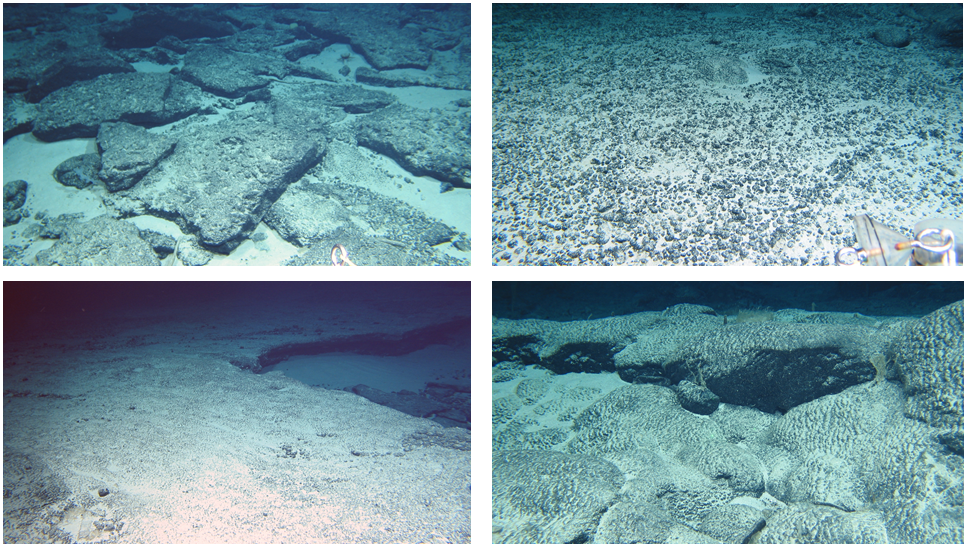
\includegraphics[width=5.5in]{./images/mehul1.png}
\caption{Different seafloor terrain at Takuyo Daigo seamount\cite{Thornton2013l}. . Clockwise, from top left: Broken slabs in sand, nodules, pillowy crusts and continuous flat crusts}
\label{f:mehul1}
\end{figure}
The complexity of seafloor topology (see Fig.~\ref{f:mehul1}) prohibits vehicles from simply landing at random locations and requires the identification and intelligent choice of landing sites. At the same time, the spatial scales relevant to AUV landing are too small to be observed by ship-board acoustic multibeam. Therefore, in order for an AUV to identify landing sites during its survey, it should be equipped with a mapping system capable of generating bathymetry with sufficiently high resolution, e.g. using light sectioning \cite{Inglis2012,Nishida2016,Bodenmann2016}. Even though landing site detection for aerial vehicles has been studied in \cite{Desaraju2014, Sharp2001}, the conditions essential for safe landing in underwater environments has not been sufficiently investigated. Simulations for control, navigation and dynamics of AUVs with landing capabilities have been reported in \cite{Wang2007, Du2012}. However, these previous works do not develop the sensing and data processing methods needed to automatically identify areas where a vehicle can land safely. Regarding methods to analyse seafloor terrains, Fourier analysis based segmentation and 3D alignment was described in \cite{Douillard2012,Douillard2013}. Other methods for surface classification using wavelets \cite{Bhandari2007} have also been described, but have not been applied to landing site identification. Early works by our group demonstrated a landing algorithm using Fourier analysis to separate flat ground surface from objects on the seafloor \cite{Sangekar2010c}. The algorithm rejected all protruding objects as non-landable areas, and only considered flat regions for landing. This work builds on our previous studies, identifying the geometric conditions where it is possible to land on protruding objects and to land on slopes, considering the vehicle's righting moment. 


The remainder of this paper is organized as follows; Section II describes the hardware requirements for landing, including the conceptual design of an underwater vehicle capable of landing and its high resolution mapping system for generating bathymetry with mm-resolution. In  Section III, the different steps of the algorithm to identify landing sites are described and demonstrated by simulating its performance on seafloor data obtained using an equivalent high resolution mapping system.  Section IV applies the algorithm to more than 1000\,m$^2$ of seafloor bathymetry obtained using an AUV during an underwater survey. Section V presents the conclusions of this work. 
% However, the large localization uncertainty \cite{Masmitja2016} associated with deep sea operations means that landing sites determined prior to deployment cannot be reached with sufficient navigational accuracy.


%************************Platform*******************************

\section{Landing hardware requirements}

\subsection{Vehicle hardware}
The hardware requirements for vehicles to perform landing operations are sufficiently different to standard vehicles to warrant specific consideration. In this work, we propose a vehicle concept with negative buoyancy during operation. This minimises the use of vertical thrusters during landing operations, allowing the vehicle to remain stationary and vibration free whilst landed and saves power. 

The features of the vehicle can be seen in the Fig.~\ref{f:mehul2}. Independent heave, surge, sway and heading control are needed to allow the vehicle to operate at low speeds manoeuvres and hover when necessary. Two horizontal thrusters provide surge and heading control. Two thrusters, inclined at $22.5^\circ$ with the vertical, control sway and heave. The inclined thrusters direct thrust away from the area directly below the vehicle to minimizing the disturbance of sand and sediments during landing. A nylon landing skid distributes the vehicle's weight and provides a stable footing when the vehicle has landed. This also provides enough clearence to protect the sensors on the the vehicle.

\begin{figure}[!ht]
\centering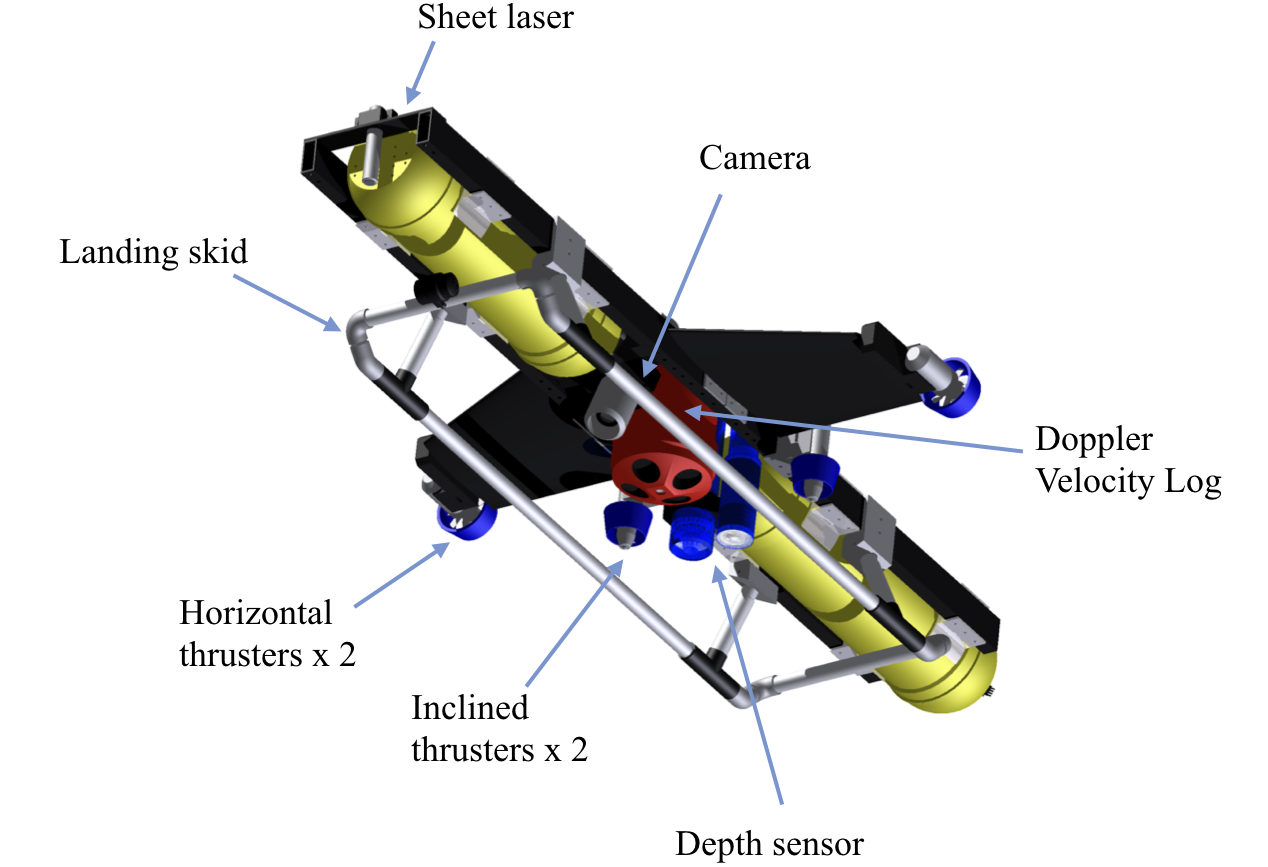
\includegraphics[width=4.5in]{./images/mehul2.png}
\caption{Concept design of a landing vehicle}
\label{f:mehul2}
\end{figure}

The vehicle is designed to be negatively buoyant to allow for landing. Although variable buoyancy engines are available \cite{Zhao2008}, these typically have a capacity of \<1\,L, and the limited change in buoyancy imposes limits on the conditions under which a vehicle can remain securely landed. Here, a hydrodynamic solution is chosen using a fixed wing NACA$651412$ profile to offset the negative buoyancy during forward motion as this approach can compensate for a large change in buoyancy. This profile produces lift at zero angle of attack and so minimising the vehicle's drag. During slow manouvres the vehicle is still able to hover, and ethods such as the two drop weight method can be used for diving and fail-safe surfacing \cite{Thornton2019}. The vehicle has a standard navigation suite, consisting of a 1.2\,MHz Doppler Velocity Log (DVL), raised more than 30\,cm of the bottom of the vehicle to provide bottom lock even when landed, a compass based Attitude Heading Reference System (AHRS), and pressure depth sensor. In addition to standard localisation, the pressure sensor and DVL range can also be used to measure vertical motion during landing and confirm the vehicle remains stationary on the seafloor once landed.

\subsection{High resolution mapping system}
\label{ssec:hres}

A high resolution mapping system using light sectioning is used to generating mm-resolution bathymetry, as illustrated in Fig.~\ref{f:mehul3}~\cite{Bodenmann2016} with associated parameters explained in Table~\ref{t:table0}. The sheet laser projects a line on the seafloor whose projection is captured by an offset camera. By detecting the laser line in the image, it is possible to determine the relative coordinates of each recognised point in the laser line. These can then be used to generate continuous bathymetry measurements in the earth-fixed coordinate system based on the vehicle's pose.

\begin{figure}[!ht]
\centering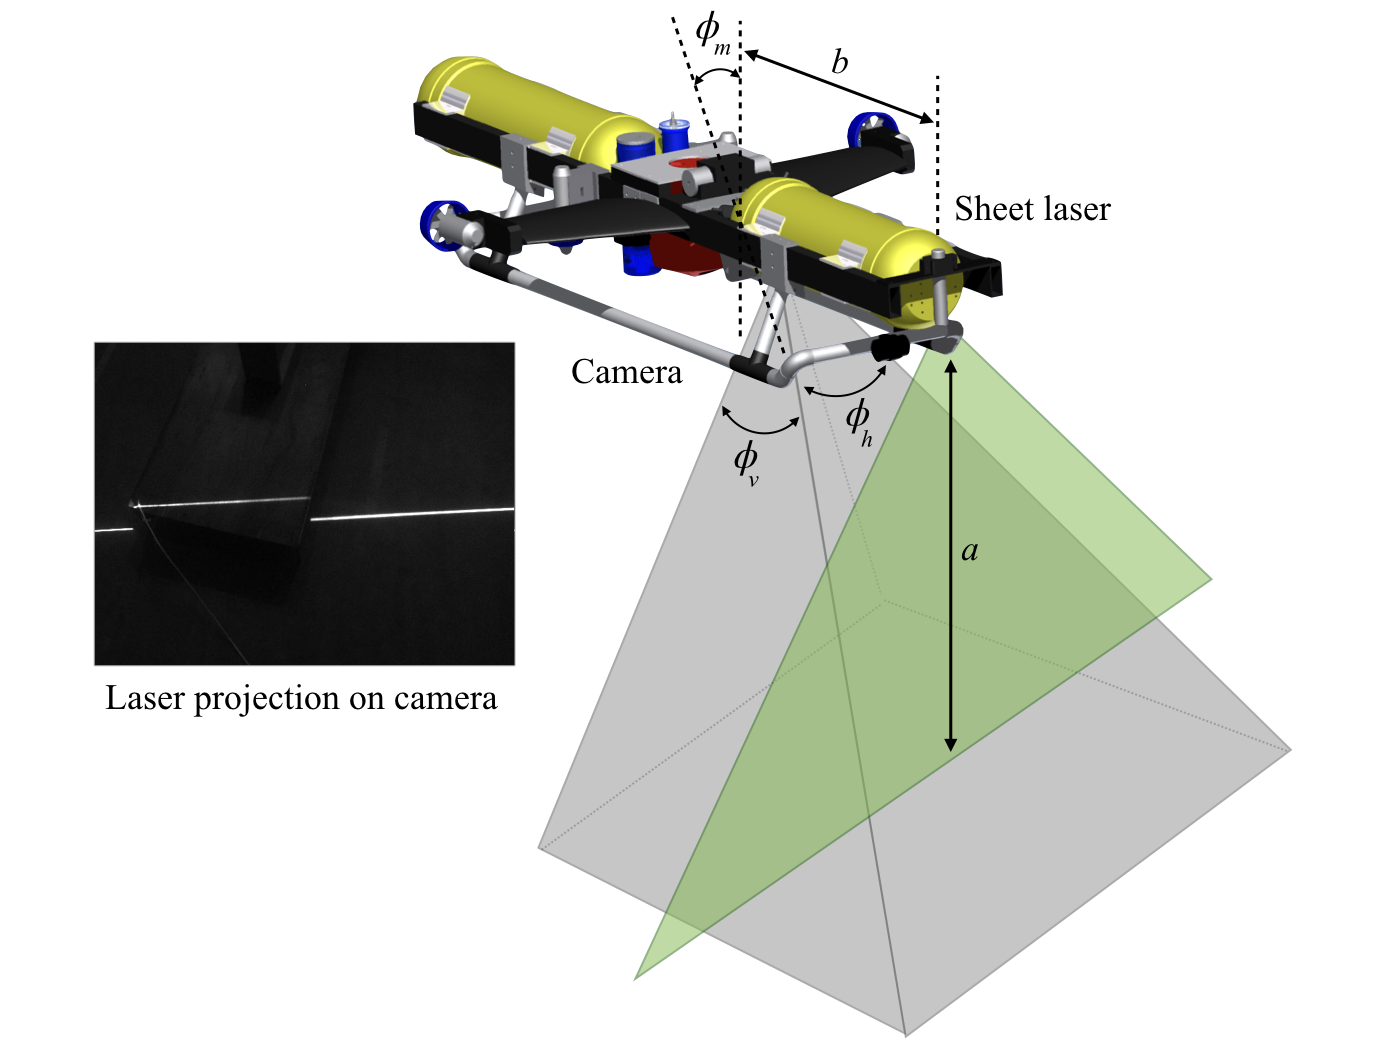
\includegraphics[width=7in]{./images/mehul3.png}
\caption{Setup and working of the high resolution mapping system}
\label{f:mehul3}
\end{figure}

\begin{table}[!ht]
\centering
\caption{Parameters of the mapping system}
\begin{tabular}{  |p{6cm}  p{4cm}| }
\hline
\textbf{Property} & \textbf{Value}\\ \hline 
Mapping altitude & $a$\\
Baseline between camera and laser & $b$\\
Vertical mounting angle of camera & $\phi_m$\\
Horizontal opening angle of camera & $\phi_h$\\
Vertical opening angle of camera & $\phi_v$\\
\hline
\end{tabular}
\label{t:table0}
\end{table}

 

%%***********************Algorithm ***********

\section{Autonomous landing algorithm}
\label{sec:algo}

The processing pipeline of the algorithm can be broken down into the following main steps.

\subsubsection{Data preprocessing} The algorithm uses high resolution point cloud generated from a mapping system as input. The preprocessing step brings the point cloud into a uniform resolution for analysis.

\subsubsection{Landing area detection}: The conditions for safe landing on the seafloor are identified for detecting a safe landing area within the point cloud. An exclusion zone is also identified where the centre of gravity of the vehicle is prohibited form landing.
 
\subsubsection{Landing site identification} Within the detected landing area, landing sites are identified which are regions where an AUV of a particular geometry can fit along a certain heading. Landing site properties are extracted for all the identified sites along different headings. 

\subsubsection{Final landing site selection} Landing costs are calculated for all the sites using the landing site properties. The site with minimum landing cost is finally selected as the final landing site.

\subsection{Data preprocessing}
\label{sub:mapping}

The algorithm requires high resolution bathymetry point cloud generated from a  mapping system as described in Section~\ref{ssec:hres}. Data was collected at a Manganese crust site on the No.$5$ Takuyo seamount by a similar mapping system mounted on the AUV BOSS-A during KR$16$-$01$ cruise of R/V Keirei, the specifications of which are given in Table.~\ref{t:table1}. Fig.~\ref{sf:mehul4a} shows a $25$ m section of the bathymetry point cloud mapped at an heading of $-130^\circ$ 

\begin{table}[!ht]
\centering
\caption{Properties of the mapping system}
\begin{tabular}{  |p{6cm}  p{4cm}| }
\hline
\textbf{Property} & \textbf{Value}\\ \hline 
Mapping altitude $a$ & $2$ m \\
Baseline between camera and laser $b$ & $1.025$ m\\
Vertical mounting angle of camera $\phi_m$ & $70^\circ$ \\
Horizontal opening angle of camera $\phi_h$ & $60.2^{\circ}$\\
Vertical opening angle of camera $\phi_v$ & $50.4^{\circ}$\\
Along-track resolution & $4$ mm\\
Cross-track resolution & $3$ mm\\
Vertical resolution & $6$ mm\\

\hline
\end{tabular}
\label{t:table1}
\end{table}

\begin{figure}[!ht]
\centering
\subfloat[Top view of seafloor color reconstruction and depth map. Black rectangles indicate areas where detailed implementation of the algorithm is shown\label{sf:mehul4a}]{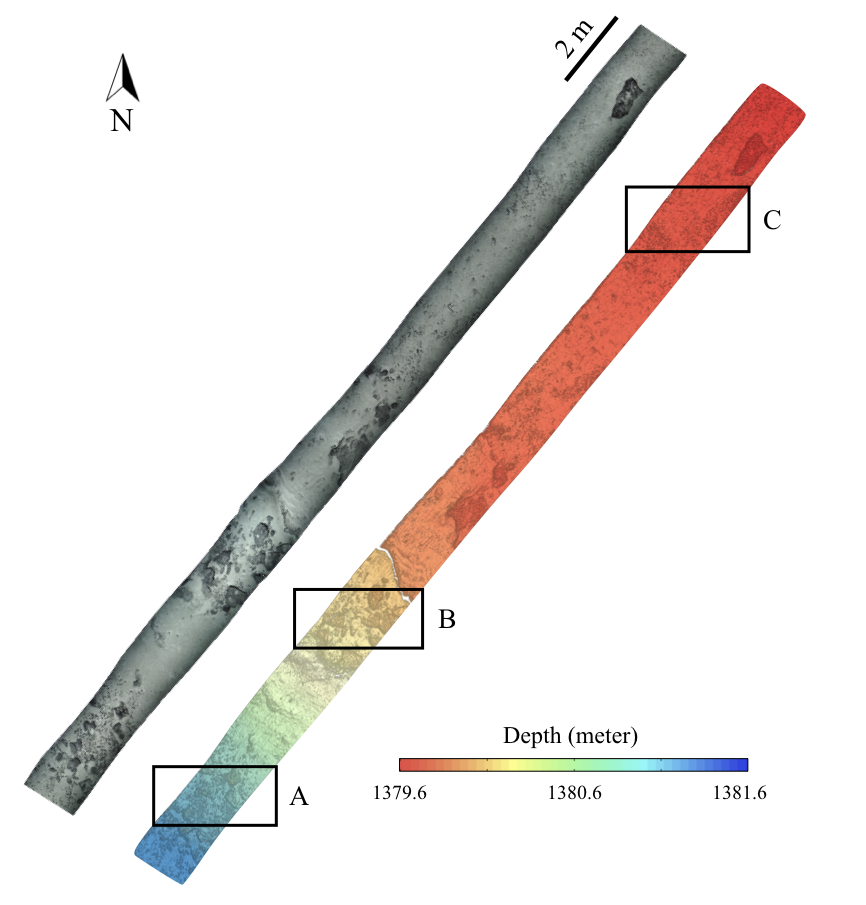
\includegraphics[width=4.5in]{./images/mehul4a.png}}\quad
\subfloat[Resampled point cloud for the three areas A,B and C\label{sf:mehul4b}]{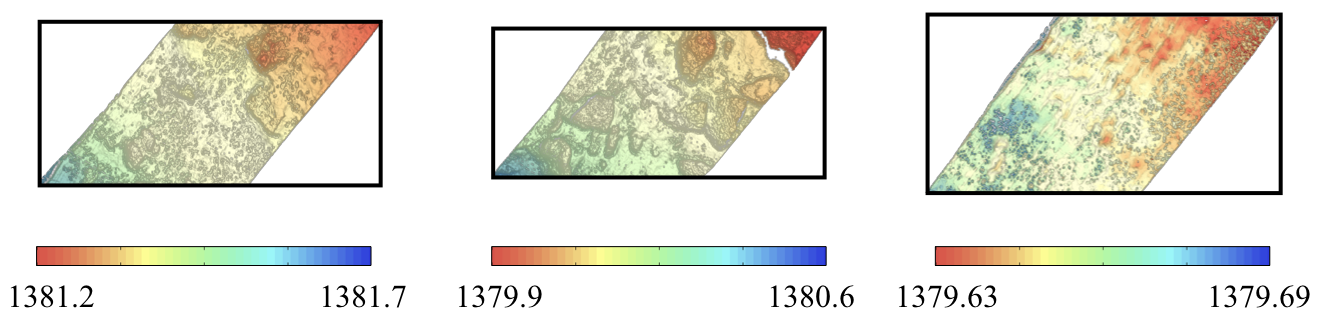
\includegraphics[width=5in]{./images/mehul4b.png}}
\caption{Seafloor bathymetry mapped using high resolution mapping system}
\end{figure}

The mapping system generates the bathymetry point cloud as northing, easting and depth. The point cloud generated from the high resolution mapping system is unstructured and resampled to a uniform grid resolution $g_{res}$. The points resampled with a resolution of $10$ mm are seen in Fig.~\ref{sf:mehul4b}. 

\subsection{Landing area detection}
\label{sub:landingarea}

Conditions for safe landing on the seafloor are determined to identify landing area in the high resolution mapped bathymetry. Landing on sloping surfaces is analyzed for the effects from the righting moment of the AUV, ground friction and seafloor currents. Analysis for safe landing on objects on the seafloor is made considering their heights. In this work, we propose the design on an AUV with negative buoyancy. AUVs are designed and navigate with their centre of buoyancy $C_B$ vertically above the centre of gravity $C_G$.  The key parameters to judge the safety of landing are given in Table~\ref{t:table2} and are defined in Fig.~\ref{f:mehul5}. The table also shows the parameter values used in the simulation of the landing algorithm.
 
\begin{table}[!ht]
\centering
\caption{Physical properties of underwater platform}
\begin{tabular}{ | p{4cm}  p{6cm} p{4cm} | }
\hline
\textbf{Property} & \textbf{Description} & \textbf{Value}\\ \hline 
$l_u$ & length of landing AUV & $1.7$ m\\
$b_u$ & width of landing AUV & $0.5$ m\\
$h_u$ & height of landing AUV & $0.45$ m\\
$F_G$ & force of  gravity (for $65$ Kg mass) & $637$ N \\
$F_B$ & force of buoyancy (for $62$ Kg mass) & $608$ N \\
$F_R$ & net  downward force  & $29$ N \\
$d_g$ & vertical distance to $C_G$ & $0.25$ m \\
$d_m$ & vertical distance between $C_G$ and $C_B$ & $0.05$ m \\
\hline
\end{tabular}
\label{t:table2}
\end{table}

\begin{figure}[!ht]
\centering
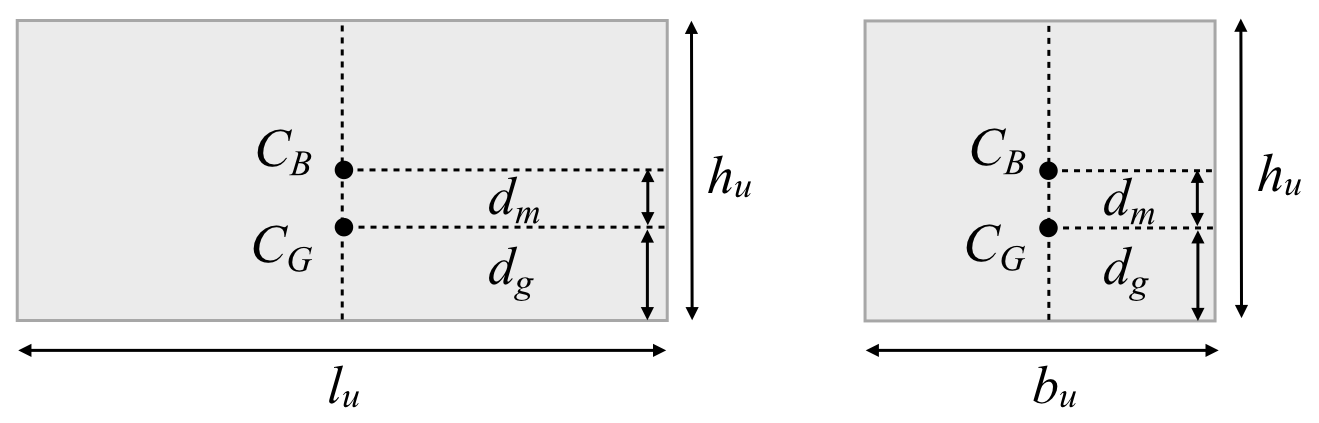
\includegraphics[width=5.0in]{./images/mehul5.png}
\caption{Side and top view of an AUV with parameters used to determine landing conditions}
\label{f:mehul5}
\end{figure}


\subsubsection{Landing on sloping surface}

When landing on a sloping surface, the AUV is considered safe when it can remain stationary and in full contact with the slope. In this work, we determine the minimum slope of the surface for the geometry of the AUV where it can meet this condition. The landing of the AUV on surface with slope is analyzed along different landing orientations of the AUV$\psi$ to find this minimum slope  $\theta_c$ as seen in Fig~\ref{f:mehul6}. 
	While landing, the AUV first makes contact with the slope along its smaller 
	edge $b_u$ for orientations $0^\circ$ and $90^\circ$ and longer edge $l_u$ 
	for orientations $180^\circ$ and $270^\circ$. For all other orientations, 
	the AUV makes contact along one of its corners.

\begin{figure}[!ht]
\centering
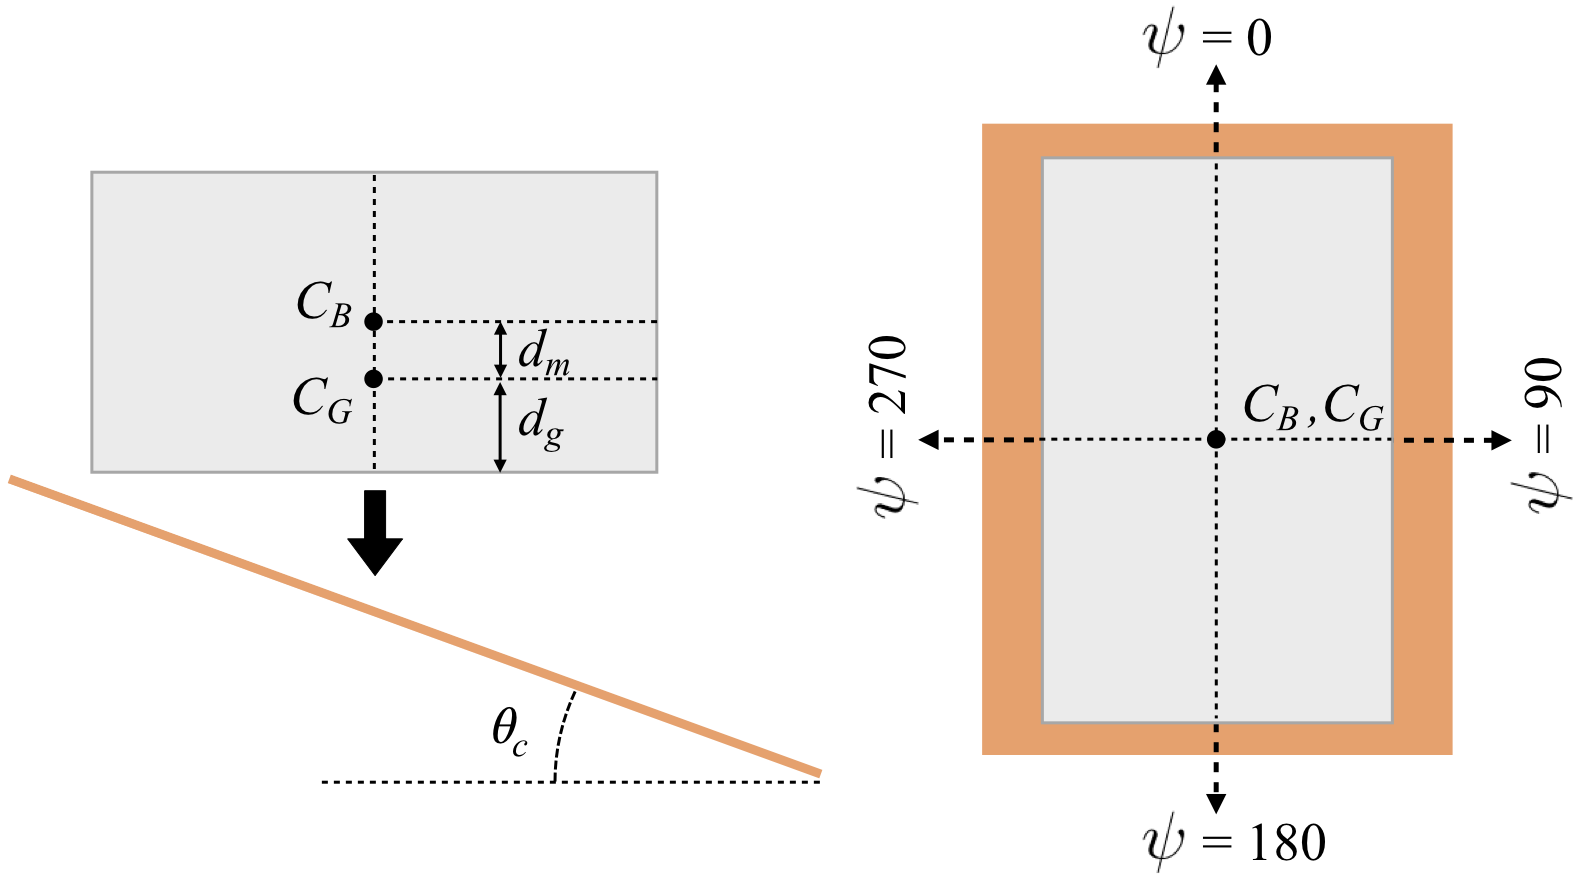
\includegraphics[width=5in]{./images/mehul6.png}
\caption{Side and top view of an AUV landing on a sloping surface}
\label{f:mehul6}
\end{figure}


\begin{figure}[!ht]
\centering
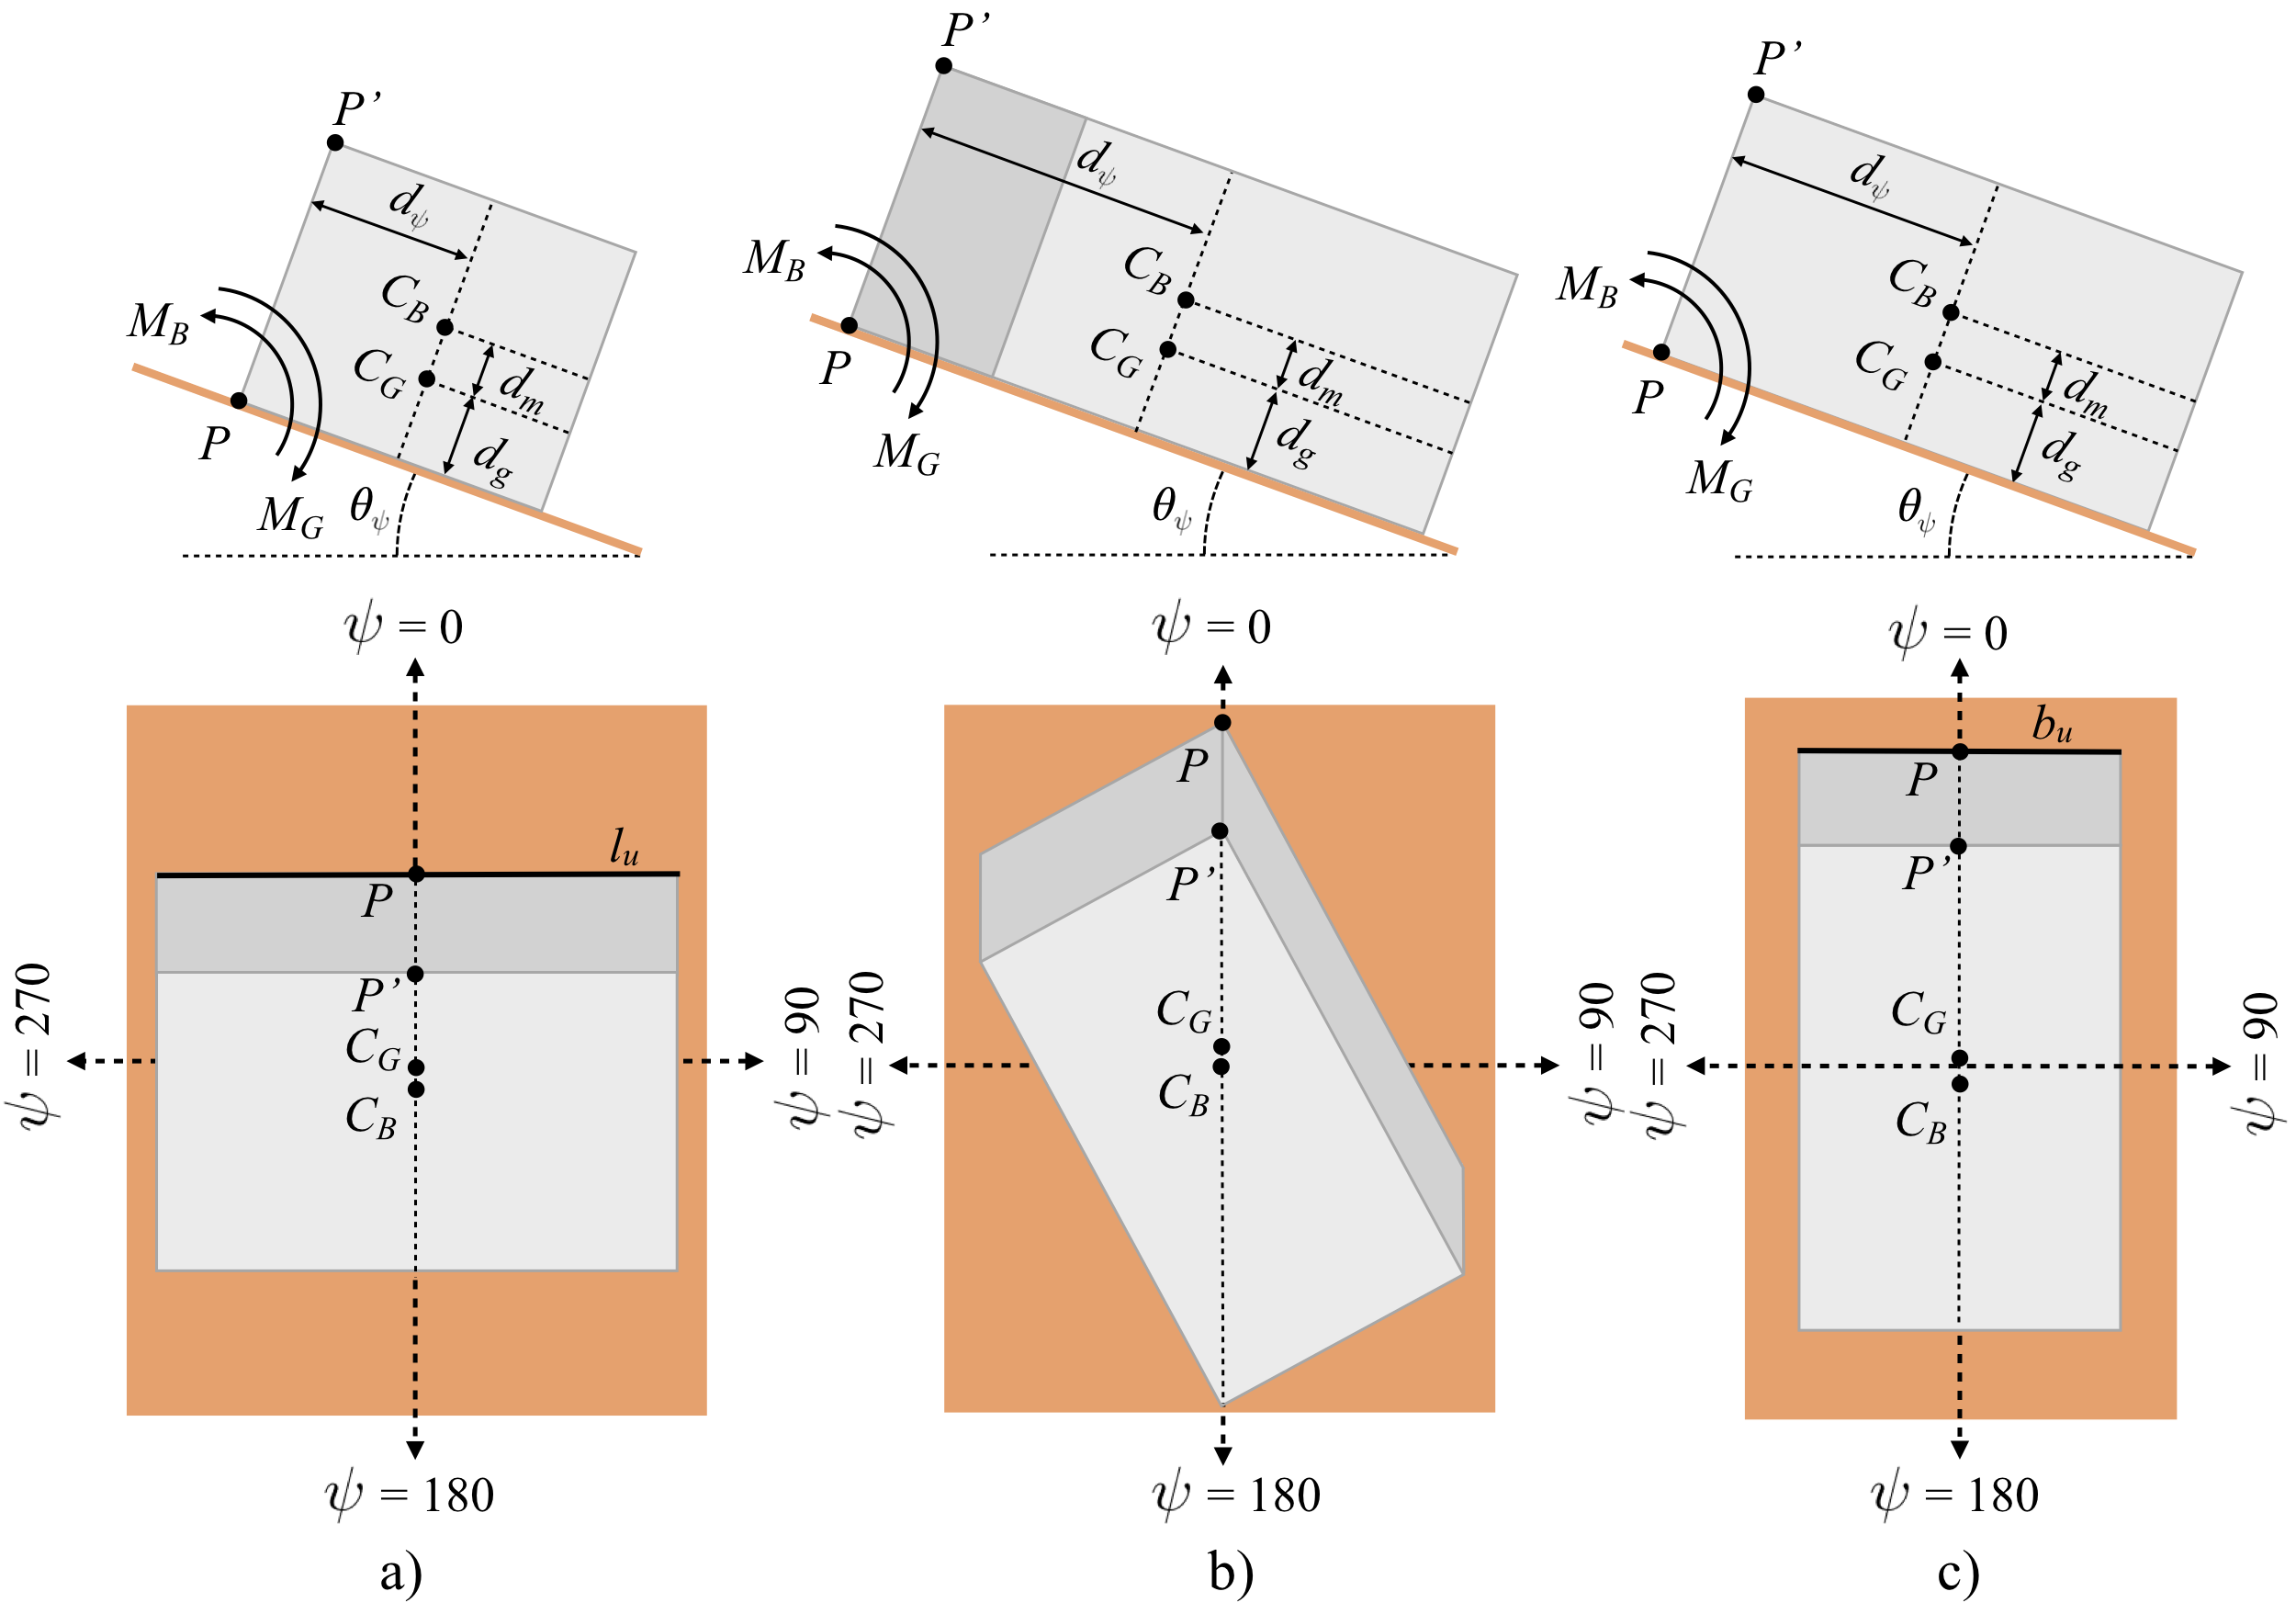
\includegraphics[width=\textwidth]{./images/mehul7.png}
\caption{AUV landing on a sloping surface along different orientations}
\label{f:mehul7}
\end{figure}

After making contact, the AUV can rotate to a maximum angle which is determined by the righting moment of the AUV. The AUV rotates along the plane formed by $C_G$, $C_B$, point $P$ and $P$' as seen in Fig~\ref{f:mehul7}. For a distance $d_{\psi}$ along landing orientation $\psi$, the maximum angle of rotation is given by the equation:

\begin{equation}
\label{eq:eq1}
\centering
	\theta_\psi = \tan^{-1}\left[ \frac{(d_{\psi} \times F_R)}{(d_m \times F_B) - (d_g \times F_R)}\right]
\end{equation}\\

For safe landing, the AUV should make contact with the ground before or at its maximum angle of rotation. While landing along its edges or when normal to the diagonal as seen in Fig~\ref{f:mehul7}, the AUV can make full contact with the surface in one stage. For other orientations, the AUV rotates until one of its edges makes contact with the slope after which it rotates about that edge to make full contact with the surface. The landing of the AUV was simulated along  orientations from $0^\circ$ to  $360^\circ$ to calculate the slope where the AUV can make full contact with the surface for each orientation as seen in Fig~\ref{f:mehul8}. Simulation was also performed for $1$, $2$ and $4$ aspect ratios of $l_u$ and $b_u$ to represent different types of underwater AUVs. From these it was determined that minimum rotation occurs when then AUV lands on its shorter edge $l_u$ as in Fig~\ref{f:mehul7}a resulting in the smallest slope of ground where the AUV can land. The minimum slope of the ground where the AUV can land safely $\theta_c$ is then calculated by using $d_{\psi} = 0.5 \times b_u$ in Equation~\ref{eq:eq1} as follows:

\begin{equation}
\label{eq:eq2}
\centering
	\theta_c = \tan^{-1}\left[ \frac{(0.5 \times b_u \times F_R)}{(d_m \times F_B) - (d_g \times F_R)}\right]
\end{equation}\\


The value of the minimum slope of the ground $\theta_c$ for the simulation using the dimensions of the AUV is calculated as $17.7^\circ$.

\begin{figure}[!ht]
\centering
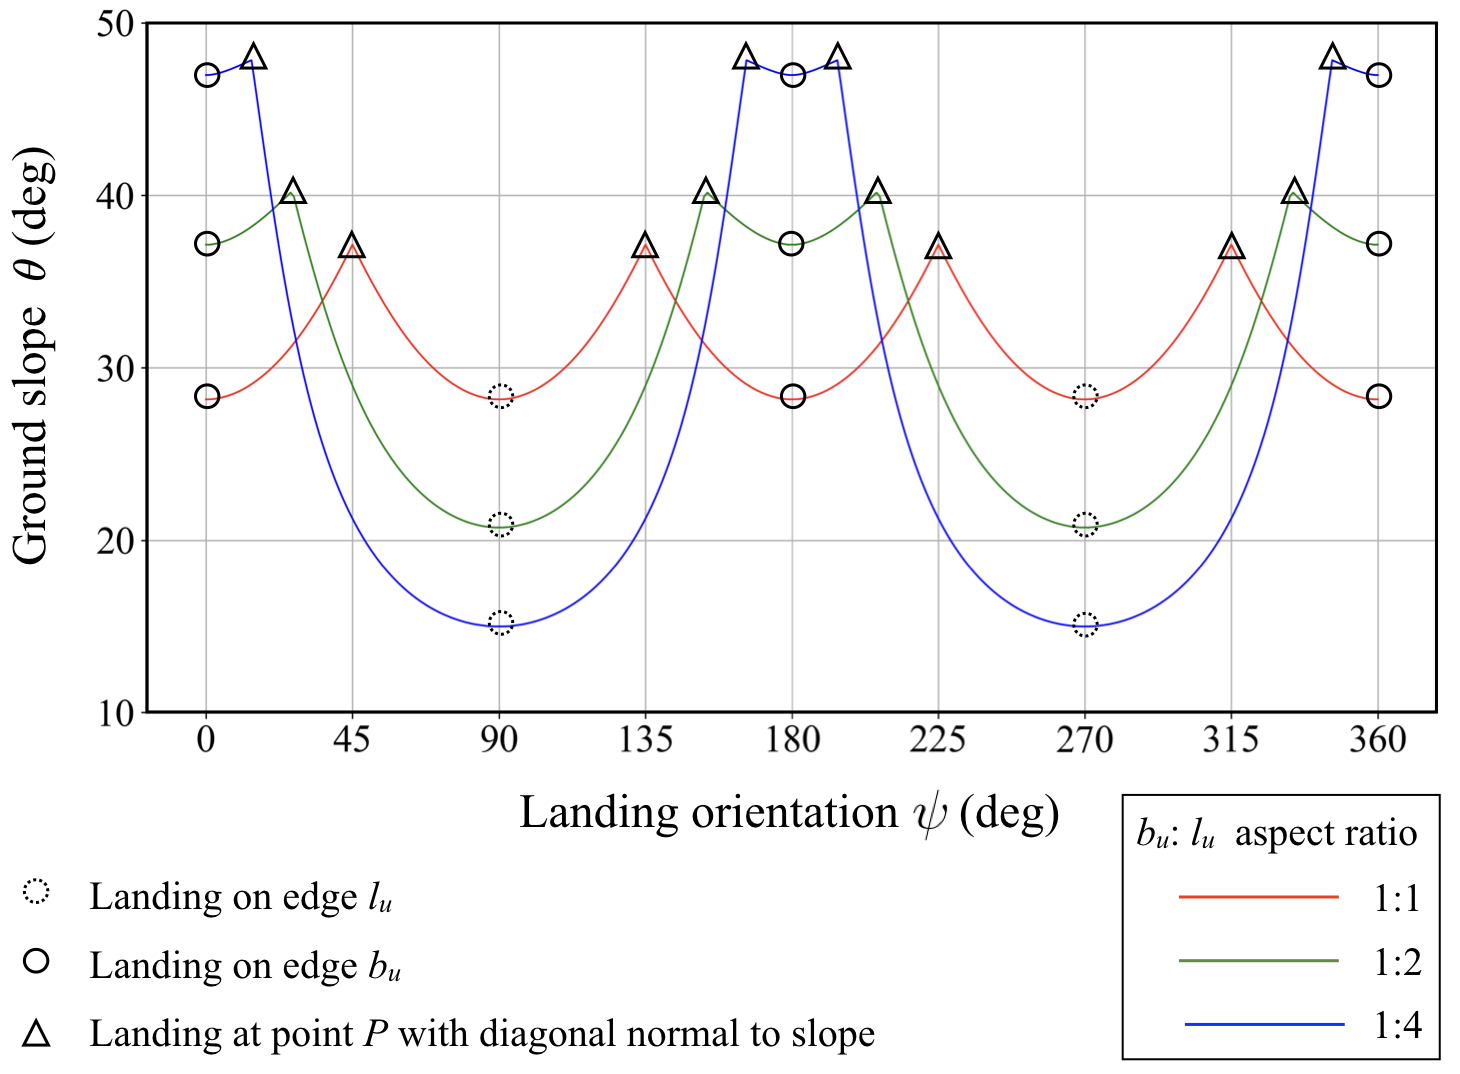
\includegraphics[width=6in]{./images/mehul8.png}
\caption{Slope calculated for different landing orientations and aspect ratios of the AUV}
\label{f:mehul8}
\end{figure}

Once landed, the AUV can remain stationary on the sloping surface if the force of friction $F_F$ counters the component of gravity $F_G$ along the slope and the force due to seafloor currents $F_C$ pushing the vehicle downslope as seen in Fig~\ref{f:mehul9}. The slope of the surface where the vehicle can remain stationary depends on the coefficient of friction $\mu$ between the AUV and seafloor. The relation between the velocity of seafloor currents $v$ and the slope at which the vehicle can remain stationary without slipping  while landing along its longer edge $l_u$ is calculated. For a drag coefficient $C_d = 1.05$ and density $\rho= 1000$ Kg/m$^3$, the velocity of seafloor currents is then calculated as:

\begin{equation}
\label{eq:eq3}
\centering
	Fc = (F_G - F_B) \times (\mu \cos\theta - \sin\theta)
\end{equation}

\begin{equation}
\label{eq:eq4}
\centering
	v_c = \sqrt{ \frac{2 \times Fc}{C_d  \times  \rho  \times  l_u \times h_u}}
\end{equation}


\begin{figure}[!ht]
\centering
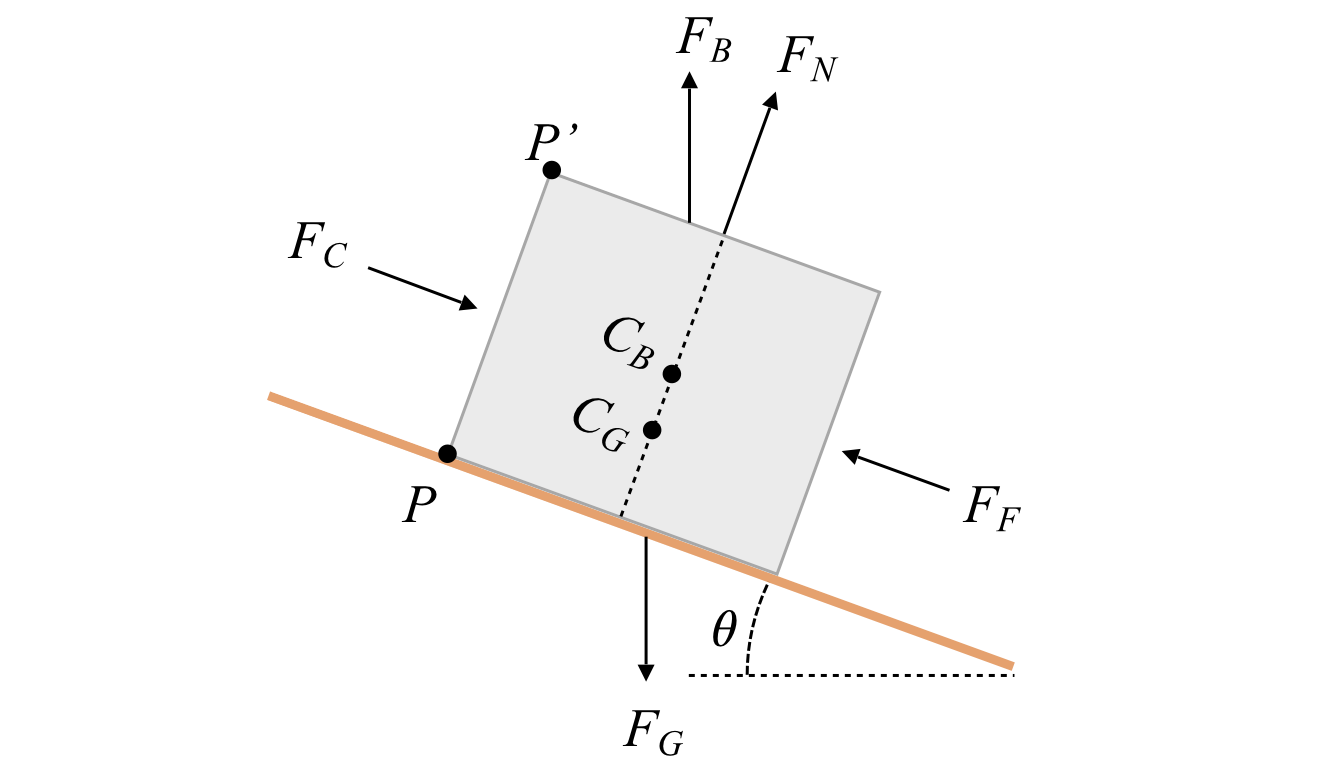
\includegraphics[width=4.8in]{./images/mehul9.png}
\caption{Forces acting on the AUV after landing on the sloping surface}
\label{f:mehul9}
\end{figure}

 Since the seafloor can have different compositions, it is difficult to estimate the exact coefficient of friction without identifying the actual nature of the seafloor. Hence, to analyze the effects of friction, current velocity values are calculated for angles between $0^\circ$ to $35^\circ$ and coefficients of friction $0.1$ and $0.6$. The values of coefficients of friction are selected based on pervious seafloor measurements ~\cite{Lambrakos1985} and seafloor currents using the Gebco database. The results indicate that the vehicle seafloor current values are within acceptable limits as seen in Fig.~\ref{f:mehul10}. 
 
\begin{figure}[!ht]
\centering
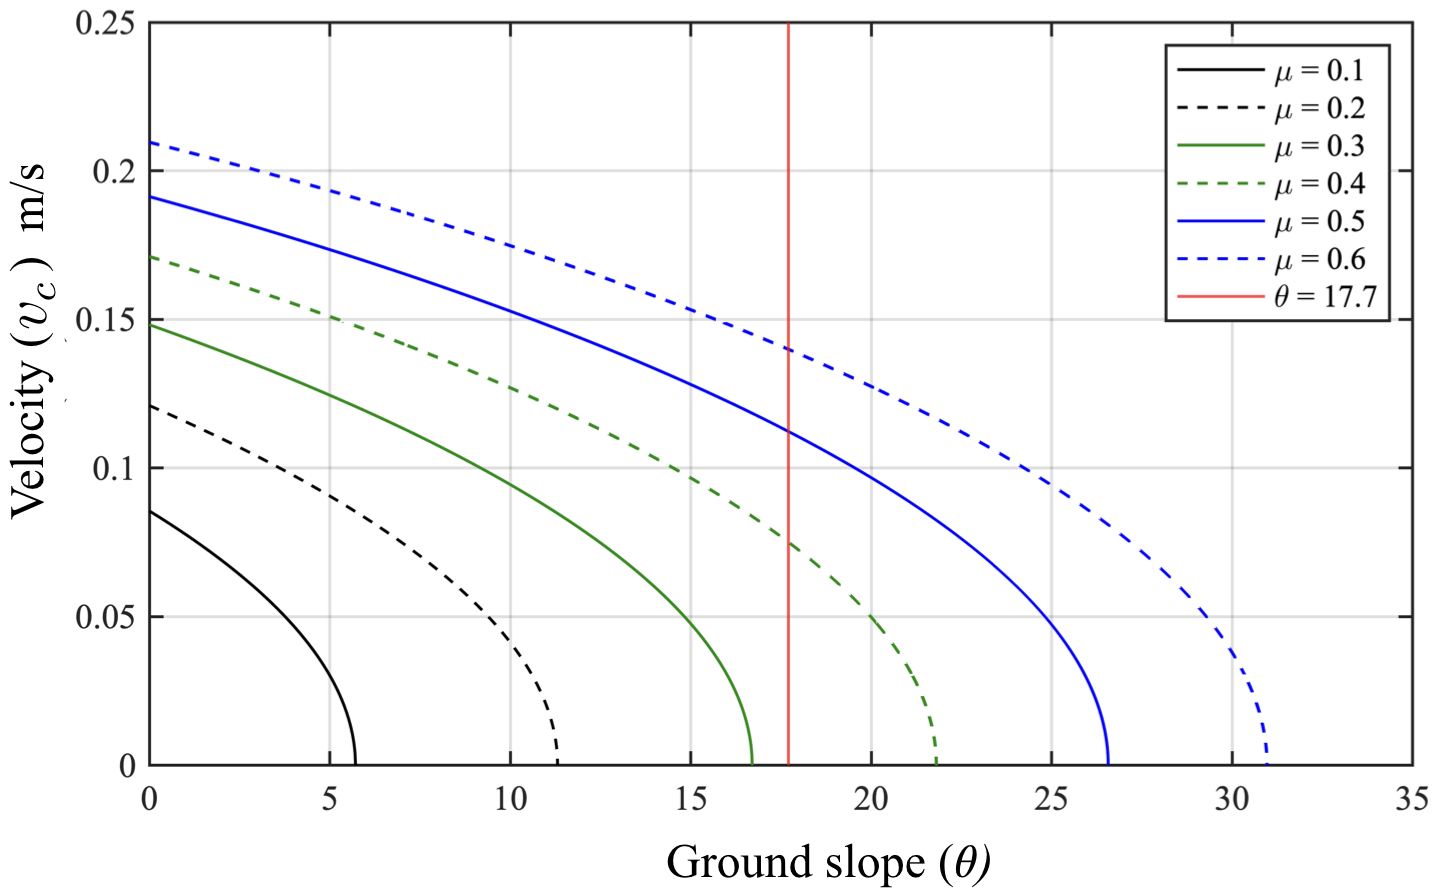
\includegraphics[width=4.5in]{./images/mehul10.png}
\caption{Analysis of seafloor currents and friction on the ground slope}
\label{f:mehul10}
\end{figure}

\subsubsection{Landing on object on the seafloor}

While landing on objects, the AUV is considered safe if the remaining part of the AUV makes full contact with the ground and is stable. Unfavorable conditions occur when the vehicle lands on an object and is partially suspended due to its righting moment. In this work, we analyze the the landing of an AUV at a point $P_i$ on the edge on an object at a distance $d_i$ from the $C_G$ of the AUV as seen in Fig~\ref{f:mehul11}a. 

\begin{figure}[!ht]
\centering
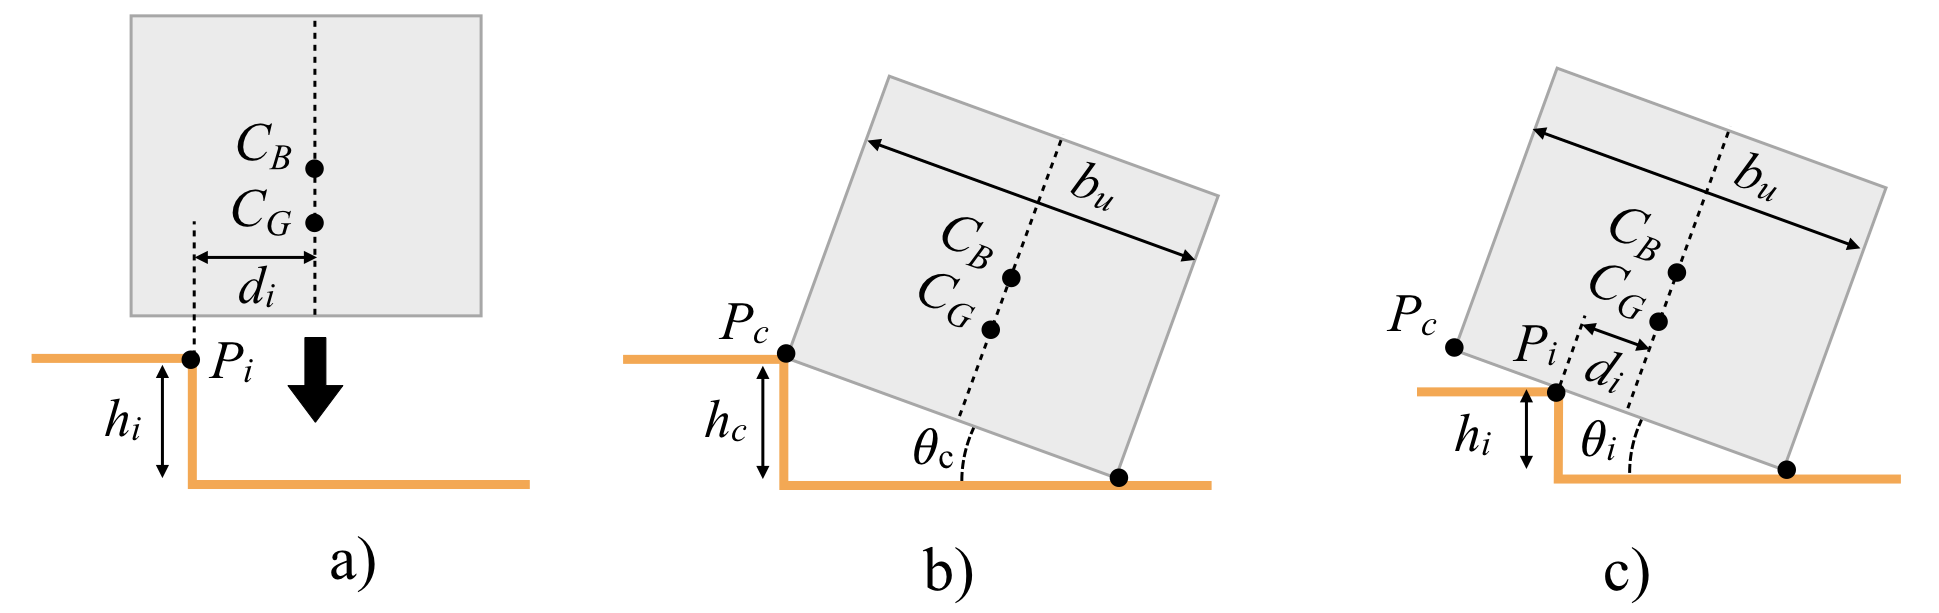
\includegraphics[width=\textwidth]{./images/mehul11.png}
\caption{a) Vehicle landing on an object on the seafloor b) Extreme condition of landing on an object c) Landing at a point between extreme condition and the centre line}
\label{f:mehul11}
\end{figure}

Extreme condition occurs when the AUV lands along its longer edge $l_u$ on the object at point $P_c$ thereby making the slope $\theta_c$ with the ground as seen in Fig~\ref{f:mehul11}b. The maximum height of the object face $h_c$ where the AUV can land safely is then calculated as:

\begin{equation}
\label{eq:eq5}
\centering
	h_c = b_u \times \sin\theta_c\
\end{equation}

The maximum height of the object face $h_c$ for our simulation is calculated as $0.152$ m. For all other points $P_i$ between $P_c$ and the $C_G$-$C_B$ centre line, we calculate the maximum angle of rotation of the AUV after making contact the object using Equation~\ref{eq:eq1} as:

\begin{equation}
\label{eq:eq6}
\centering
	\theta_i = \tan^{-1}\left[ \frac{(d_i \times F_R)}{(d_m \times F_B) - (d_g \times F_R)}\right]
\end{equation}\\

from where we can calculate the maximum height of the object face for distance $d_i$ as:

\begin{equation}
\label{eq:eq7}
\centering
	h_i = (0.5 \times b_u + d_i)\times \sin\theta_i
\end{equation}


\begin{figure}[!ht]
\centering
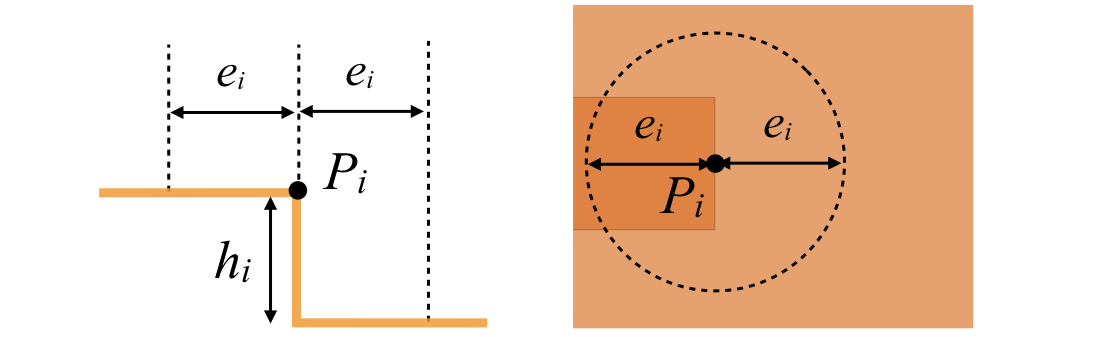
\includegraphics[width=4.5in]{./images/mehul12.png}
\caption{$C_G$ exclusion where the centre of gravity of the AUV is prohibited from landing}
\label{f:mehul12}
\end{figure}


This allows us to create a $C_G$ exclusion zone $e_i$ of size $d_i$ around each face of the object with height $h_i$ where the $C_G$ of the AUV is prohibited from landing as in Fig~\ref{f:mehul12}. The $C_G$ exclusion zone calculated in steps of $5$ mm equivalent to the mapping resolution for the dimensions of the AUV is seen in Fig~\ref{f:mehul13}.

\begin{figure}[!ht]
\centering
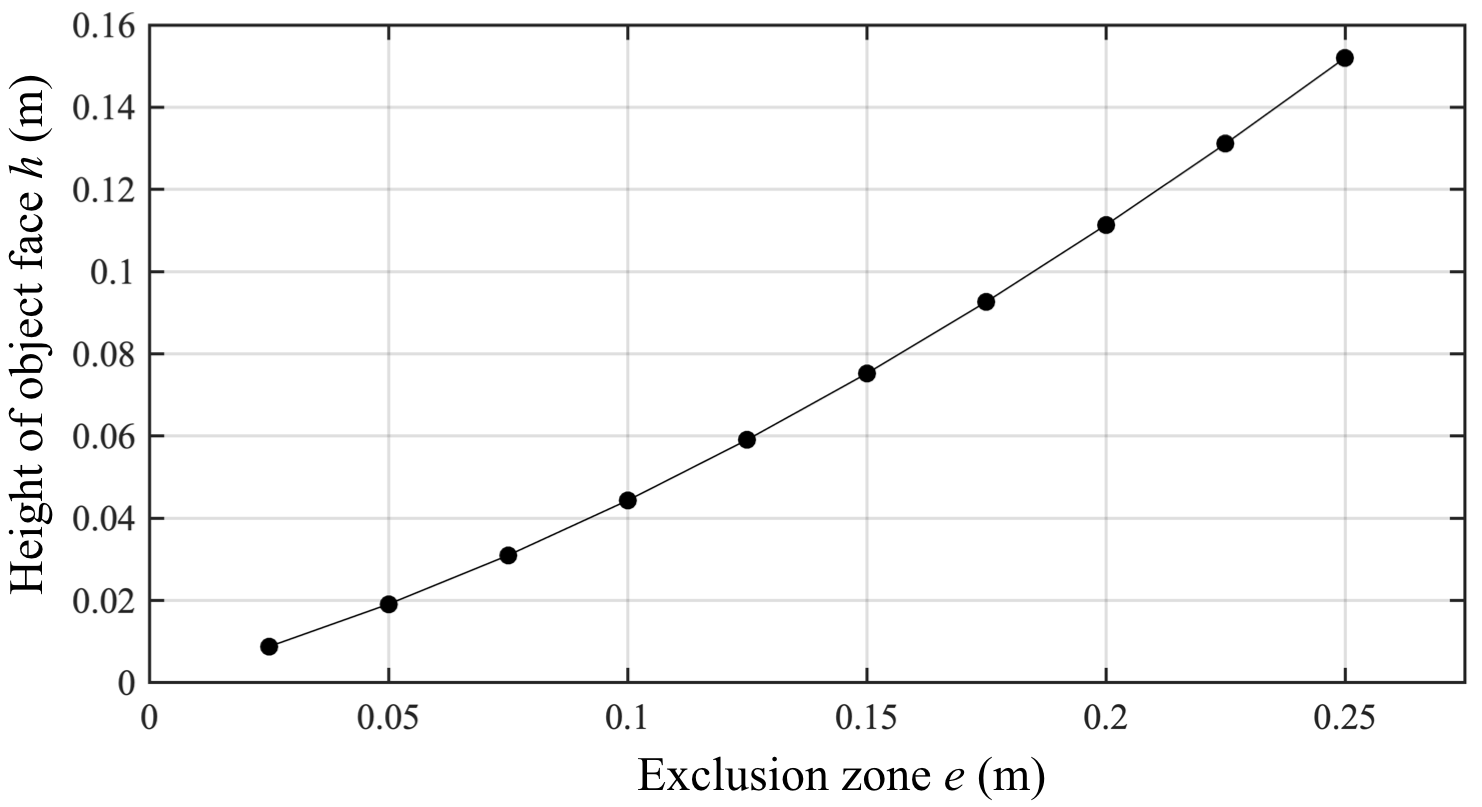
\includegraphics[width=5.5in]{./images/mehul13.png}
\caption{Exclusion zone for height of objects faces}
\label{f:mehul13}
\end{figure}

The vehicle should be prohibited from landing on object faces with height more than $h_c$ requiring a $C_G$ exclusion zone of size half the diagonal of the AUV in all directions. However, since most AUVs are not circular in shape, the $C_G$ exclusion zone for these points can be calculated based on the geometry of the AUV and the heading during landing $\alpha$. This will also reduce the size of the $C_G$ exclusion zone.  Using the conditions identified for safe landing, the flowchart of the algorithm for landing area and exclusion zone detection is seen in Fig~\ref{f:mehul14}.

\begin{figure}[!ht]
\centering
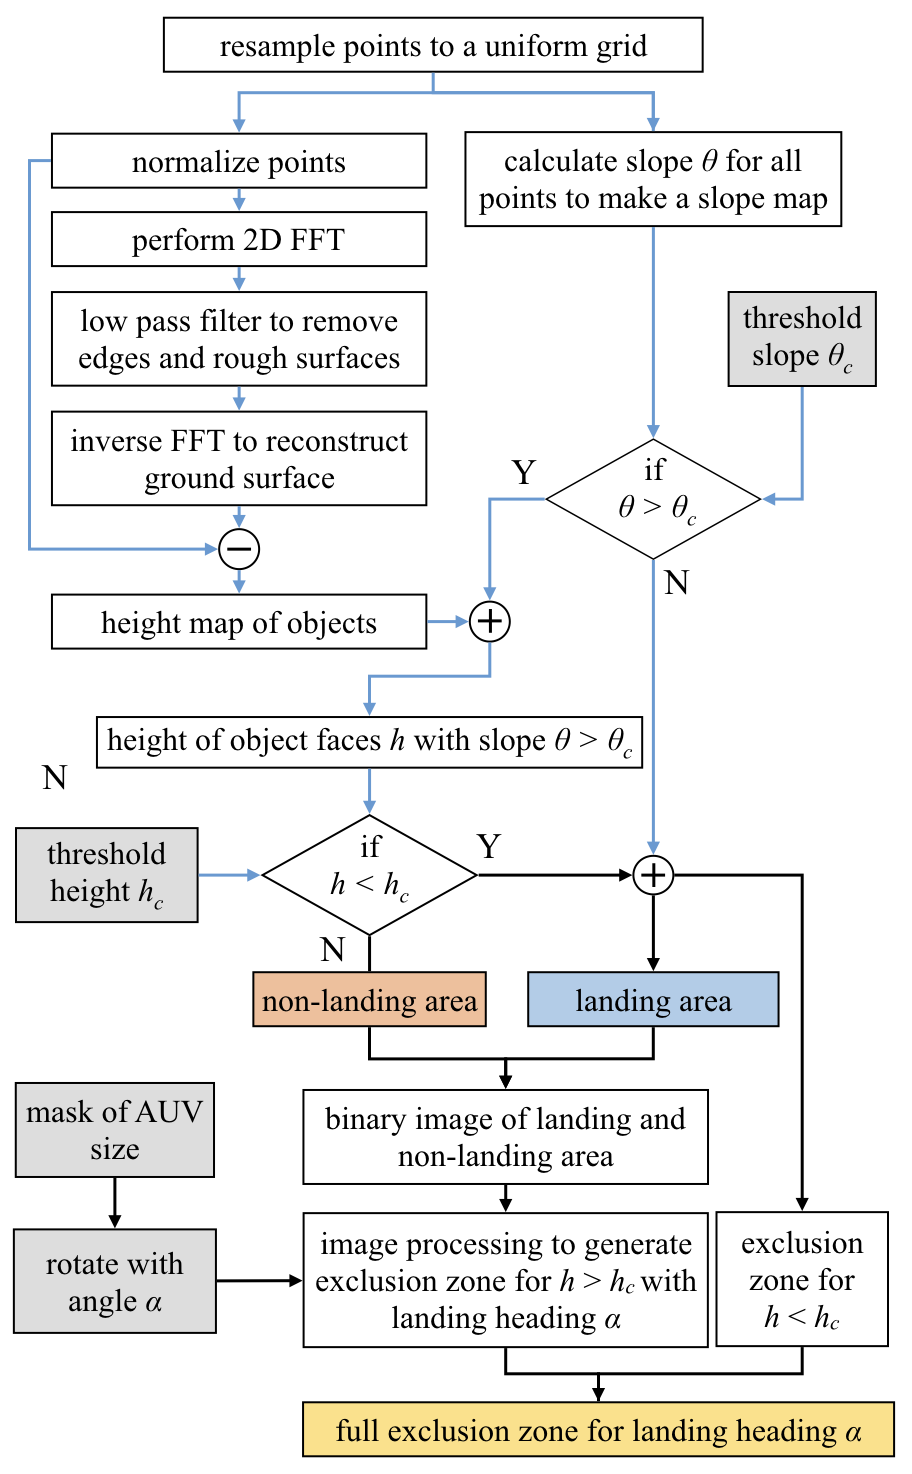
\includegraphics[width=4in]{./images/mehul14.png}
\caption{Flowchart for detection of landing area and generation of $C_G$ exclusion zone}
\label{f:mehul14}
\end{figure}

\subsubsection{Processing point cloud}


A slope map is generated for the resampled point cloud. Two vectors are computed from three neighboring points making a triangle whose cross product is taken to find the normal vector. The angle of this normal vector to the horizontal is then calculated as the slope. Slope map generated for the three areas A,B and C is seen in Fig.~\ref{f:slope_analysis}a. Slope threshold $\theta_c$ is applied to the slope map to generate a binary slope threshold map. The slope threshold map for $h_c = 17.7^\circ$ for the simulation is seen in Fig.~\ref{f:slope_analysis}b.

\begin{figure}[!ht]
\centering
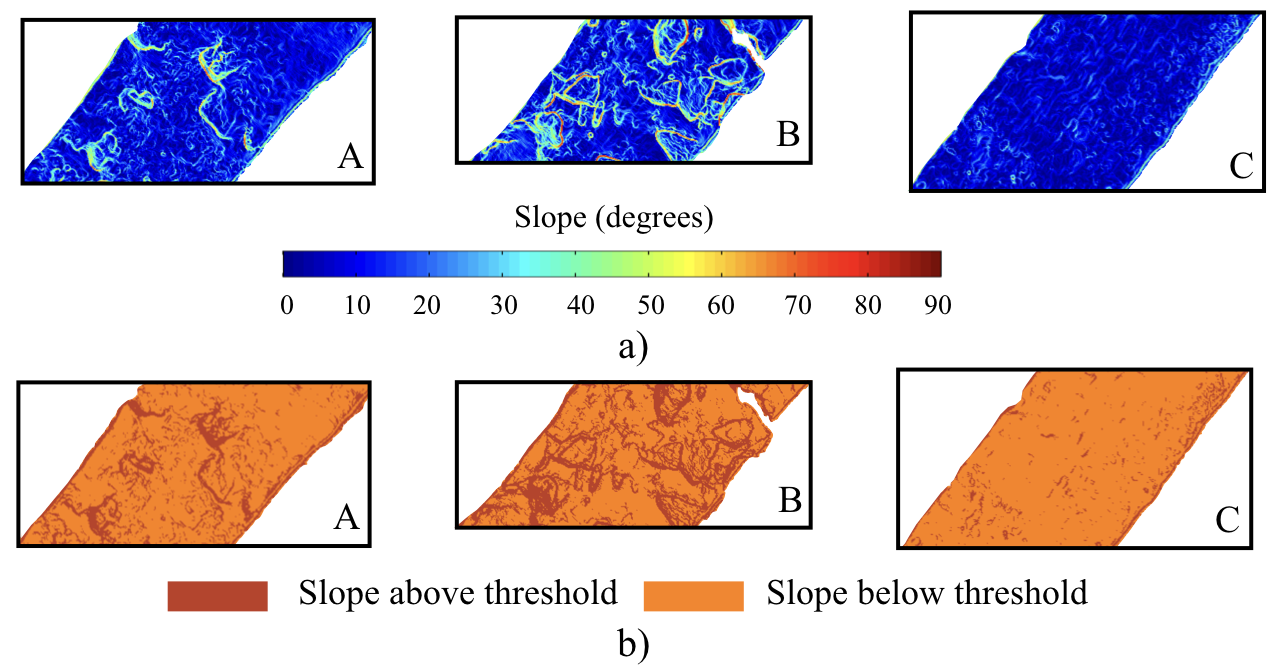
\includegraphics[width=6in]{./images/mehul15.png}
\caption{a) Slope calculated for areas A B and C. Area B shows objects having faces with higher slope than block C and A. Area C shows more smoother surface with less slope b) Slope threshold map for the three areas }
\label{f:slope_analysis}
\end{figure}

Laser projections of different seafloor terrain show distinctive profiles. The frequency content of these profiles is analyzed for separating objects from the ground surface. Flat areas are dominated by low frequency components of the profiles while the high frequency components represent the sharp edges of objects and rough surfaces. Analysis is performed on in each area using a two dimensional Fast Fourier Transform (FFT). The points in the area are zero filled on all sides to form a $N \times N$ matrix, where $N$ is the next power of $2$ more than the largest dimension of the area. The depth values of the points are then normalized to remove the DC component by subtracting the mean depth value and rotated along their Eigenvectors. Two dimensional $N$ point FFT is performed on the normalized values to convert them to frequency domain values. The frequency bins are $n \times f_s/N$, where $n = 1, 2, \dots, N/2$ and $f_s = 1/g_{res}$ the sampling frequency. A low pass filter with a linear phase response with nearly even response in the pass band and a sharp cut-off is applied to the frequency domain values to suppress the high frequency components. For cut-off frequency $f_c$, filter order $n$ and frequency bins $f$, the equation of the filter used is:

\begin{equation}
\label{eq:eq8}
\centering
	h_{l}(f) = \frac{1}{\sqrt{1 + (\frac{f}{f_c})^{2n}}} 
\end{equation}

A filter order of $3$ is used to provide suitable sharpness of damping. The filter provides a $3$ dB attenuation at the cut-off frequency. To decide the cut off frequency we identify the minimum size of the object considered as ground. For an object of size $\sigma$, represented by a step function, the equivalent sync function in frequency domain has first zero crossings at $2/\sigma$ ~\cite{Lyons1997} ~\cite{Kalogerakis2010}. The cut-off frequency is set as $f_c = 2/\sigma$ which indicates the frequency represented by the size of the object at the sampling resolution. $f_c = 5$ is used in this work. The filter function is rotated around the zero frequency to form a $N\times N$ point filter and multiplied to the frequency domain values element by element. An inverse two dimensional FFT produces smoothened values representing the ground surface. The normalized point cloud is compared to the ground surface to generate a height map of objects as seen in Fig.~\ref{f:mehul19}.

\begin{figure}[!ht]
\centering
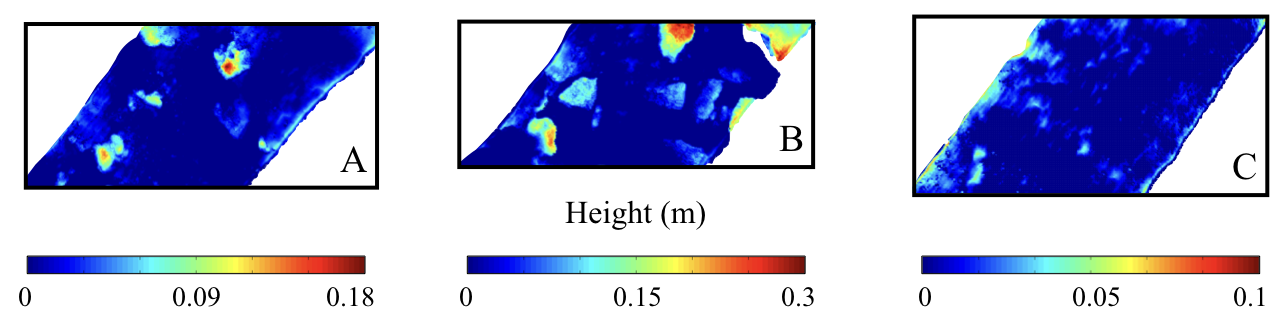
\includegraphics[width=6in]{./images/mehul19.png}
\caption{Height map for areas A B and C. Areas A and B show large objects on the seafloor compared to area C}
\label{f:mehul19}
\end{figure}

Height of object faces $h$ is extracted in areas above the slope threshold $\theta > \theta_c$ from the height map of objects as in Fig.~\ref{f:mehul20}b. A $C_G$ exclusion zone is generated for object faces with height less than height threshold $h < h_c$, using values calculated from Equation~\ref{eq:eq6} and~\ref{eq:eq7} and shown in Fig.~\ref{f:mehul13}. For this, location of all points having a certain height range are identified to form a binary image. Morphological dilation is then performed on this binary image using a circular structural element with radius equal to size of the exclusion zone for that height. Object faces with height above the threshold $h > h_c$ are identified to make a binary image with non-landing and landing area. Landing area identified for height threshold of $0.152$ m is seen in Fig.~\ref{f:mehul21}a. Since the AUV can land along different headings, the $C_G$ exclusion zone for object faces above height threshold is made taking into account the landing heading $\alpha$ and the geometry of the AUV. For this, a rectangular structural with dimensions in pixels equal to the size of the AUV is generated. The structural element is then rotated to the landing heading to generate a new structural element representing the rotated AUV.


\begin{figure}[!ht]
\centering
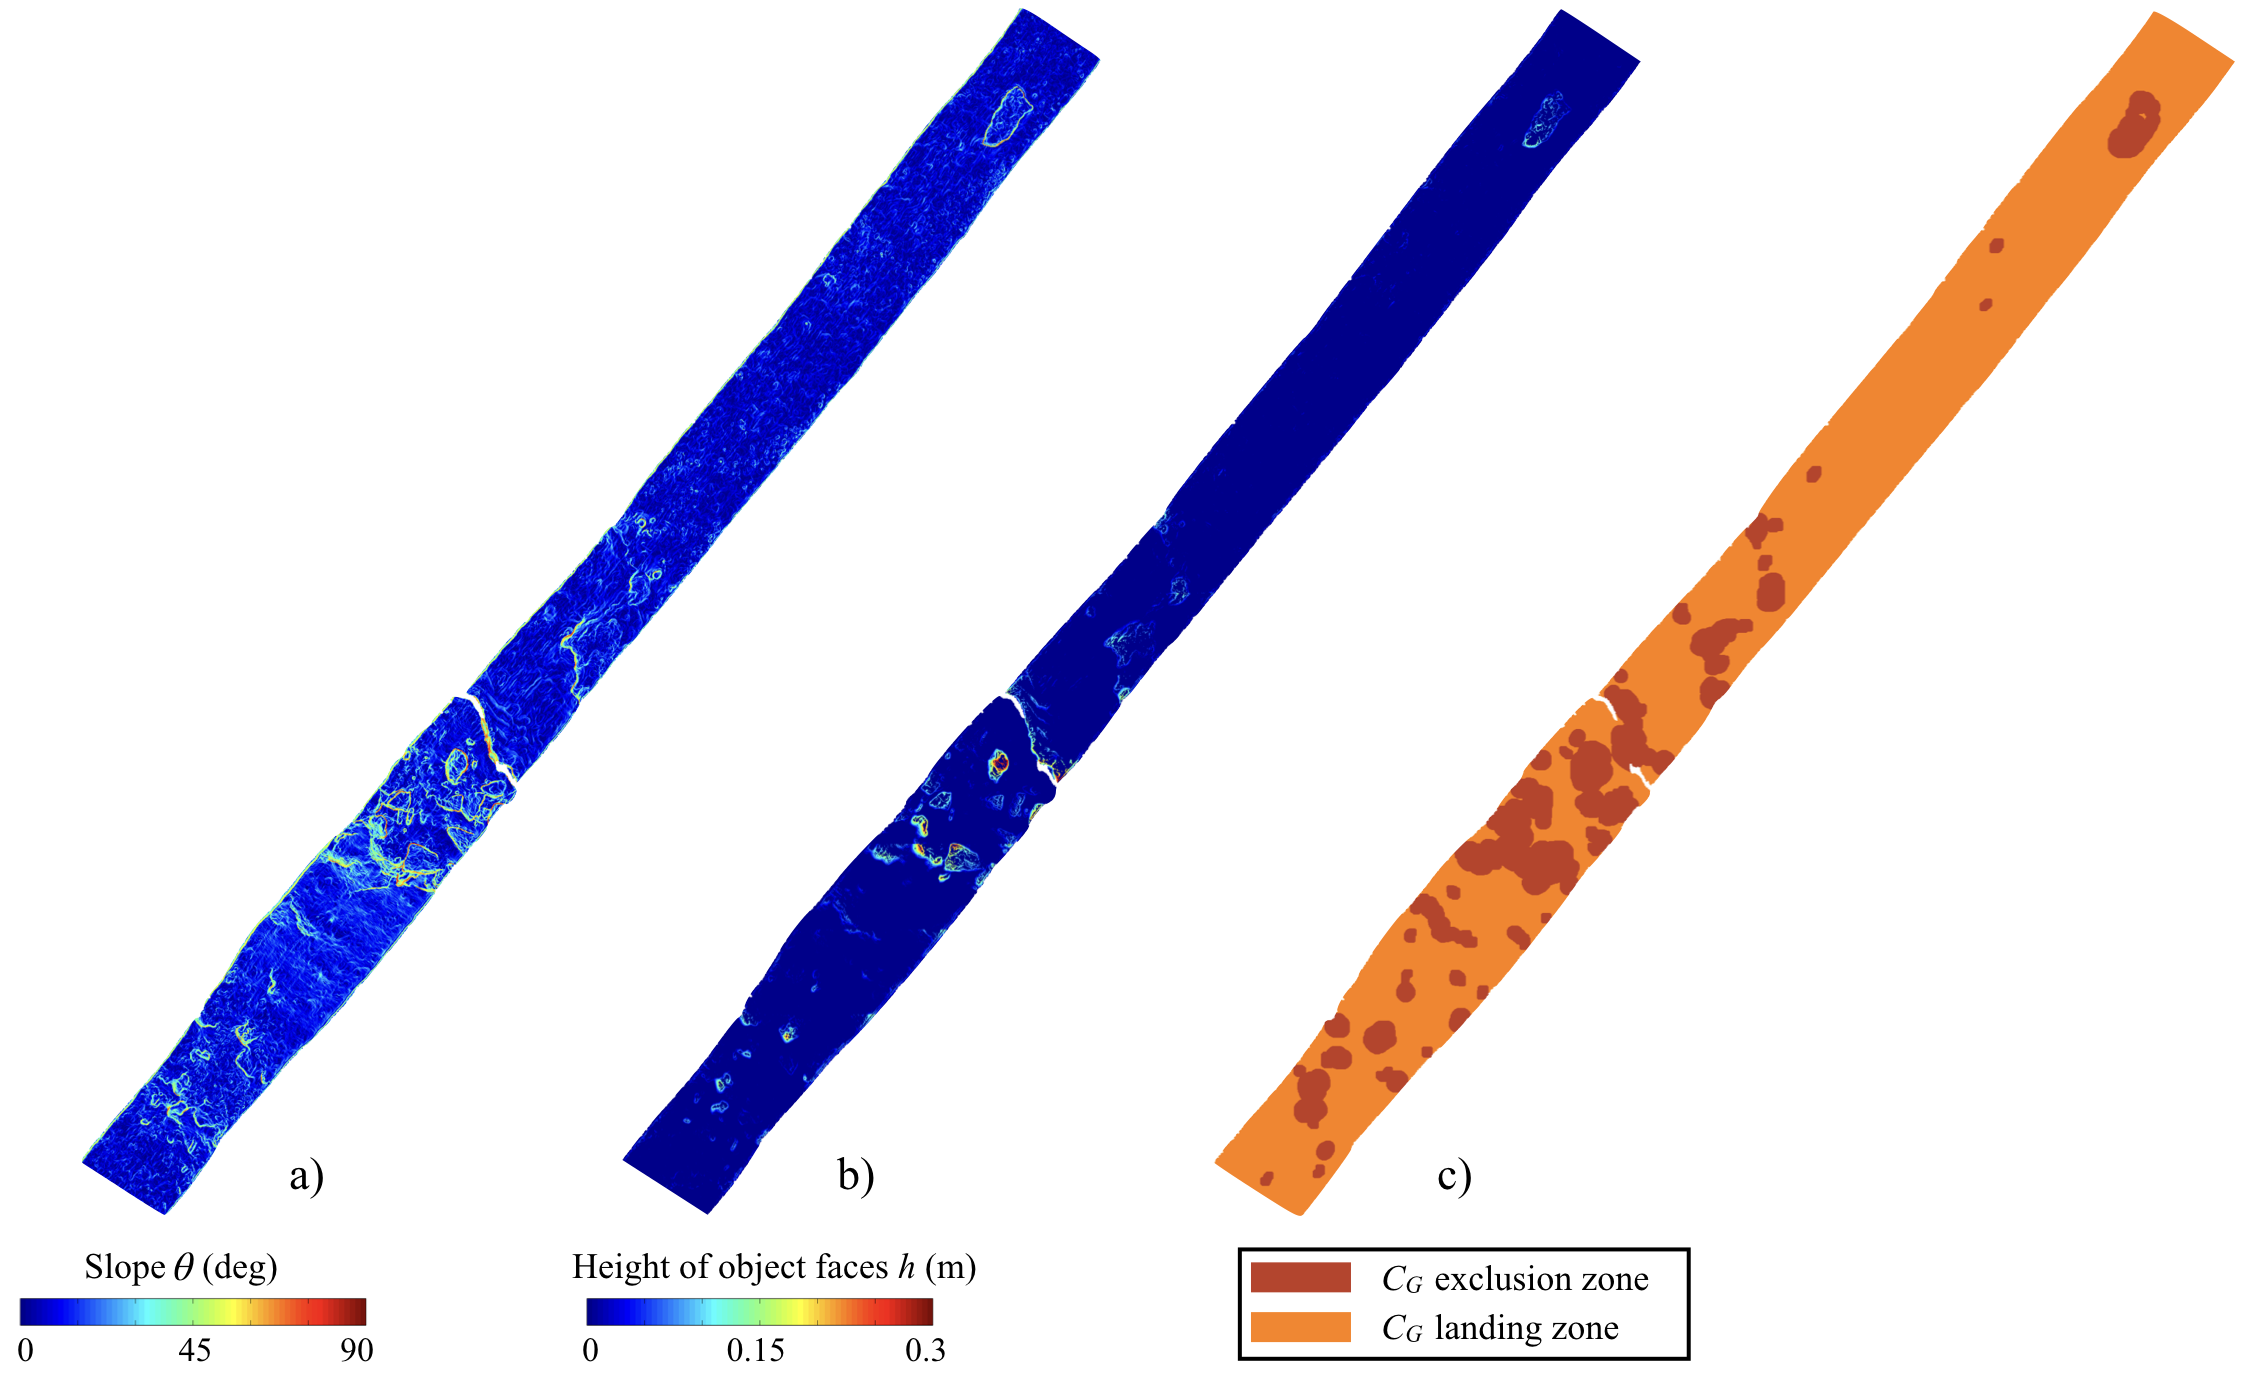
\includegraphics[width=5.5in]{./images/mehul20.png}
\caption{a) Slope map of the mapped bathymetry b) Height of object faces $h$ for slope $\theta > \theta_c$ c) $C_G$ exclusion zone for object faces $h < h_c$}
\label{f:mehul20}
\end{figure}

\begin{figure}[!ht]
\centering
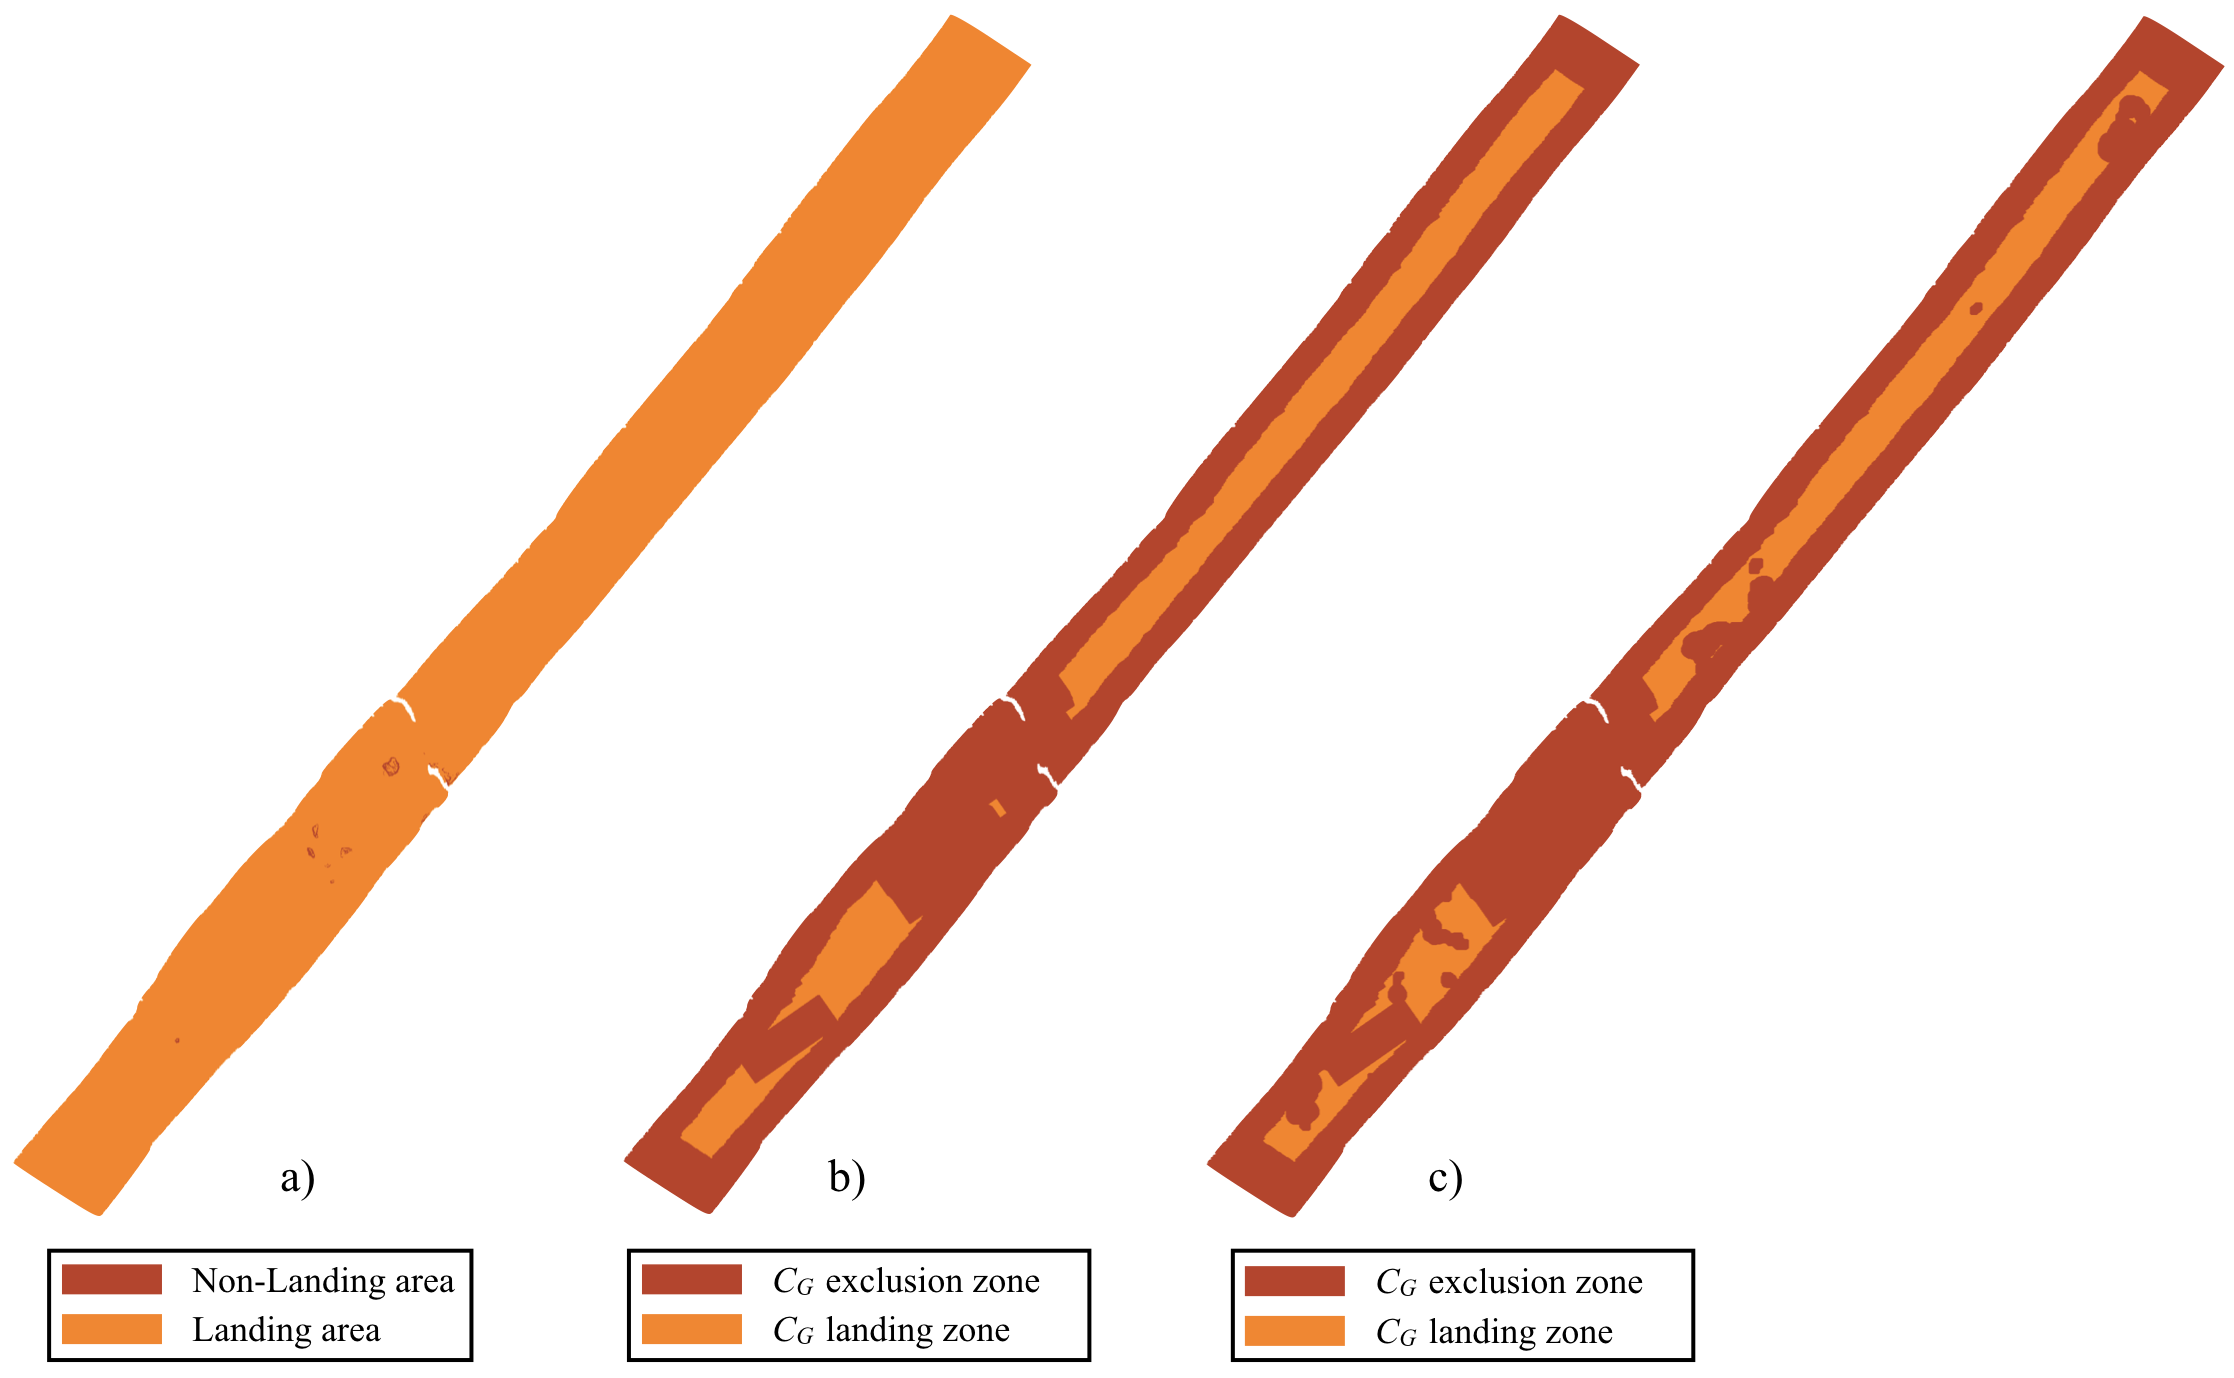
\includegraphics[width=5.5in]{./images/mehul21.png}
\caption{a) Landing area for height threshold $h > h_c$ b)  $C_G$ Exclusion zone for landing area with $55^\circ$ landing heading  c) Full $C_G$ exclusion zone for object faces $h < h_c$ and landing area with $55^\circ$ landing heading}
\label{f:mehul21}
\end{figure}

 Image opening is performed between the rotated structural element and the binary image to find area where the AUV can fit in the landing area. The points are further eroded using the rotated structural element to find area where the $C_G$ of the AUV can land. The remaining are marked as  $C_G$ exclusion zone for the landing heading. $C_G$ exclusion zone for a landing heading of $55^\circ$ is as seen in Fig~\ref{f:mehul21}b. This exclusion zone is then combined with that generated for object faces with height less than height threshold $h < h_c$ to make a full $C_G$ exclusion zone as seen in Fig~\ref{f:mehul21}c. 
 
\subsection{Identifying landing sites}

Landing sites are identified where the AUV can fit and safely land along a landing heading. For each heading, area other than the $C_G$ exclusion zone, $C_G$  landing zone is split into grounds based on eight neighboring connected pixels. Each group is identified as a landing site. The three landing sites identified for the landing heading of $55^\circ$ can be seen in Fig~\ref{f:mehul22}a.

\begin{figure}[!ht]
\centering
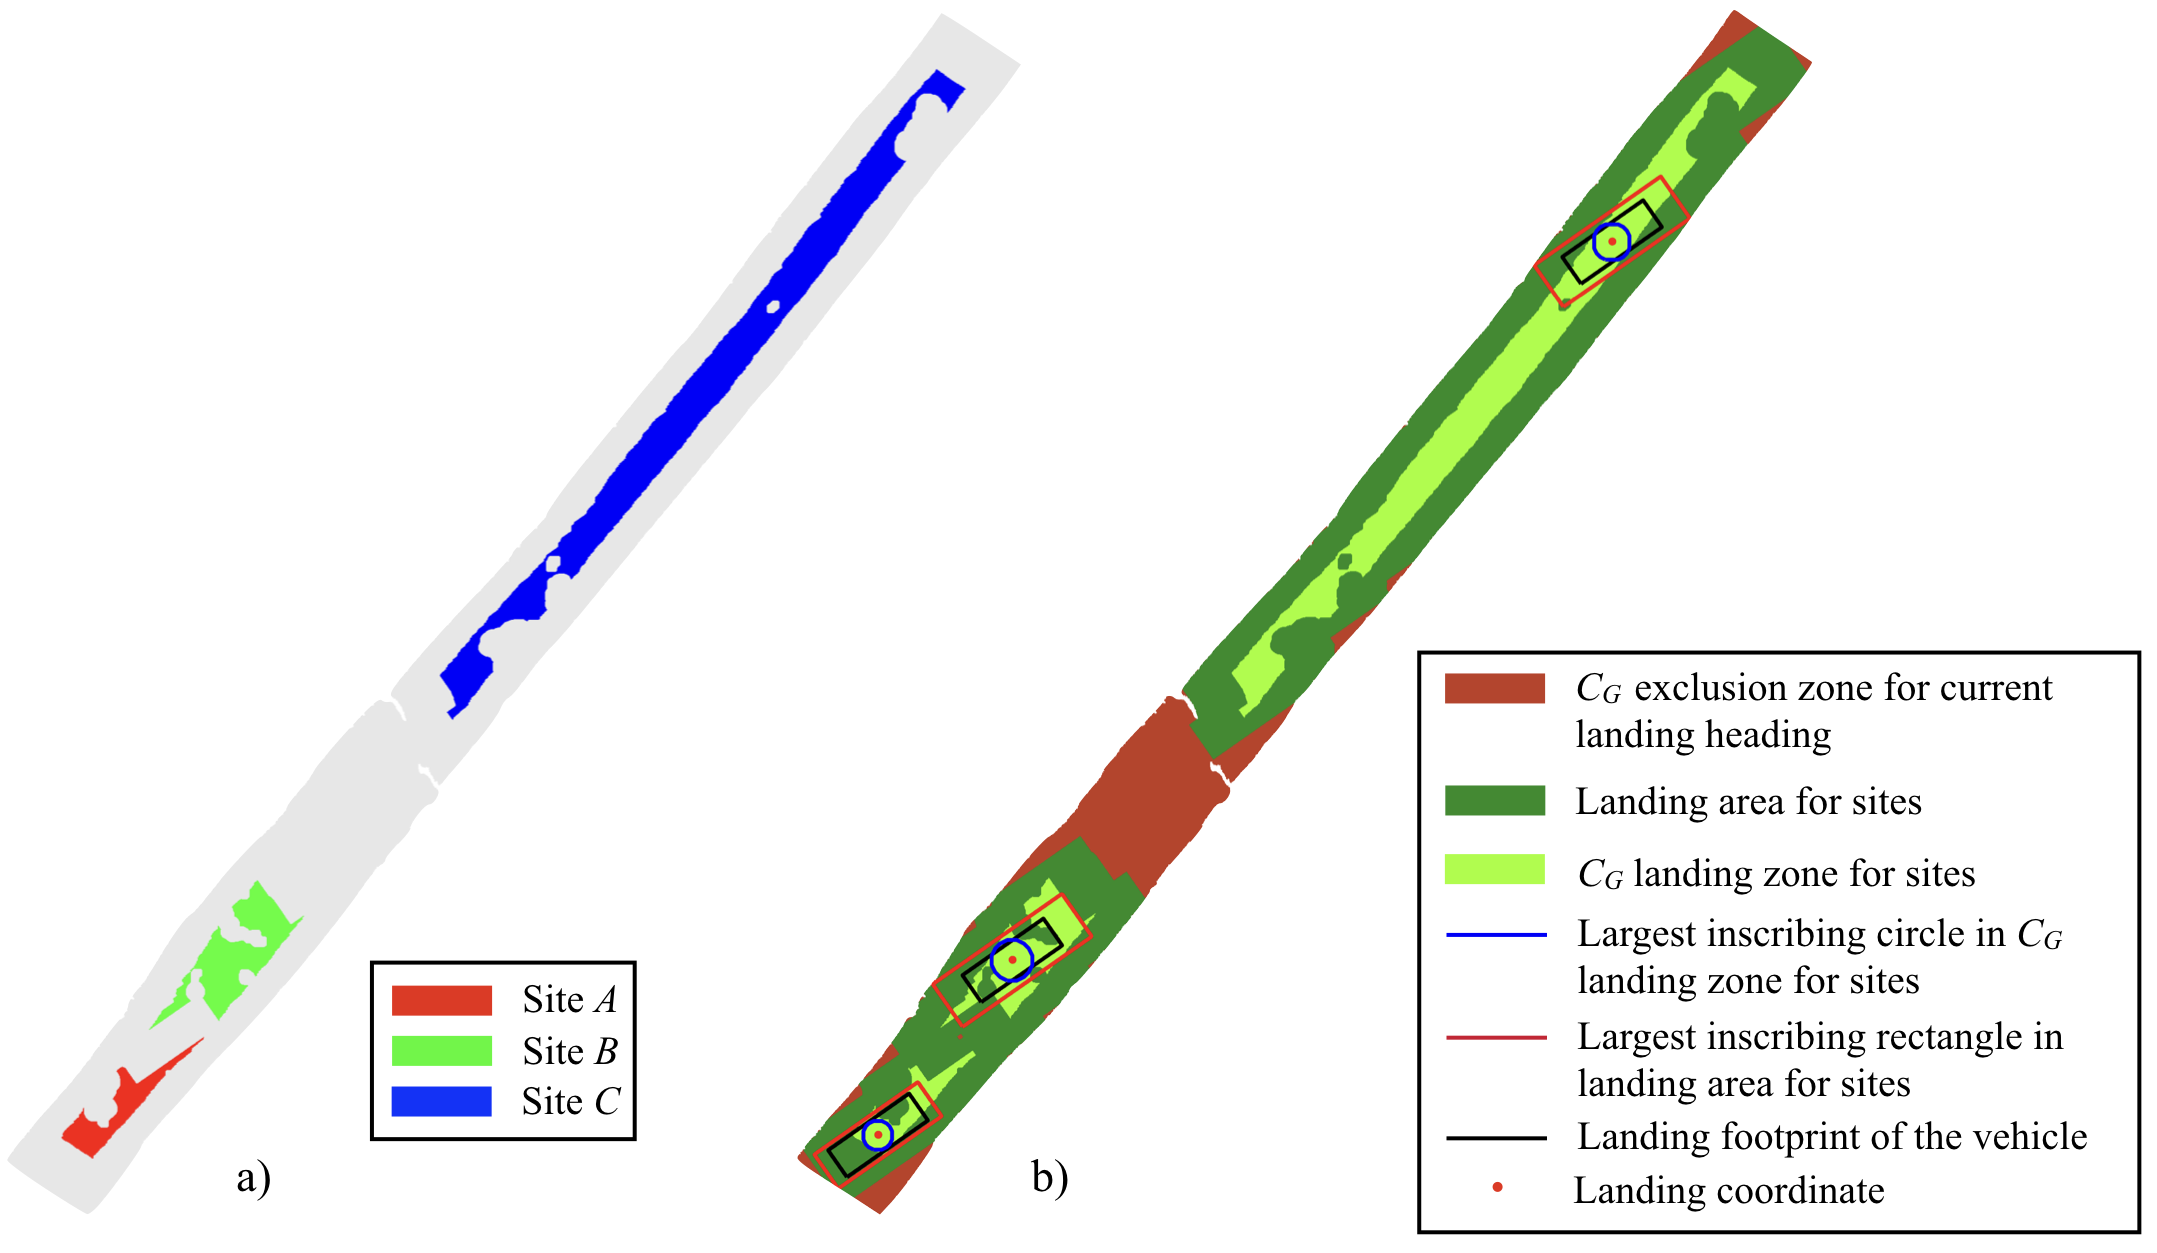
\includegraphics[width=6in]{./images/mehul22.png}
\caption{a) Landing sites identified for $55^\circ$ landing heading  b) Landing point calculation }
\label{f:mehul22}
\end{figure}

	Small groups of points are rejected since the are too small for the AUV to 
	relocate and navigate for landing due to positioning errors. A landing 
	coordinate is calculated for each site where the AUV can land furthest away 
	from the boundary of the site. For this, the largest circle that can be 
	inscribed in the site is calculated and centre of this circle is taken as 
	the landing coordinate. The footprint of the vehicle around the landing 
	coordinate along the landing heading is generated to form a rectangle where 
	the properties of the landing site are extracted. The landing coordinates 
	calculated for the site along landing heading of $55^\circ$ are seen in 
	Fig~\ref{f:mehul22}b. The following properties of the landing site are 
	extracted:\\
	
\subsubsection{Site slope $P_s$}  The mean landing slope $\overline{\theta}$ is calculated for the points in the landing footprint of the AUV. The slope is then normalized using the threshold slope $\theta_c$ to get the value of $P_s$: 
	
\begin{equation}
\label{eq:eq9}
\centering
	P_s = \frac{\overline{\theta}}{\theta_c}
\end{equation}
	
\subsubsection{Site safety $P_f$} A safety factor is calculated for the landing point which indicated how far the vehicle is from the edges of the landing site. For each site, the landing area for that site is calculated by morphological dilation of the site using the rotated structural element. The largest rectangle around the landing coordinate that can be inscribed within this landing area having same aspect ratio and landing heading as the vehicle is calculated. The ratio of area of this rectangle $A_r$ to the footprint of the vehicle $A_f$ is calculated as a safety ratio. Since values above a certain limit do not provide any additional safety, the safety ratio is limited to $5$. The value of $P_f$ is then calculates as:

 \begin{equation}
 \label{eq:eq10}
    P_f = \frac{1}{4}\left( 5 - \frac{A_r}{A_f}\right) 
  \end{equation}
	
 \subsubsection{Site roughness $P_r$} Roughness value $R$ is calculated for area under the the vehicle footprint as the average deviation of the height values $h$ from the mean $\overline{h}$. This value is then normalized by comparing with the maximum possible roughness for any terrain under the vehicle footprint $R_m$. Since the landing coordinate is not included in the $C_G$ exclusion zone, the worst case scenario of the height map is as seen in Fig.~\ref{f:mehul22a}. The roughness calculated for this is $R_m = 0.03$.

\begin{equation}
 \label{eq:eq11}
	R = \frac{1}{n} \sum_{i=1}^{n}\left | h_i - \overline{h} \right |
\end{equation} 

\begin{equation}
 \label{eq:eq12}
	P_f = \frac{R}{R_m} 
\end{equation}\\ 

\begin{figure}[!ht]
\centering
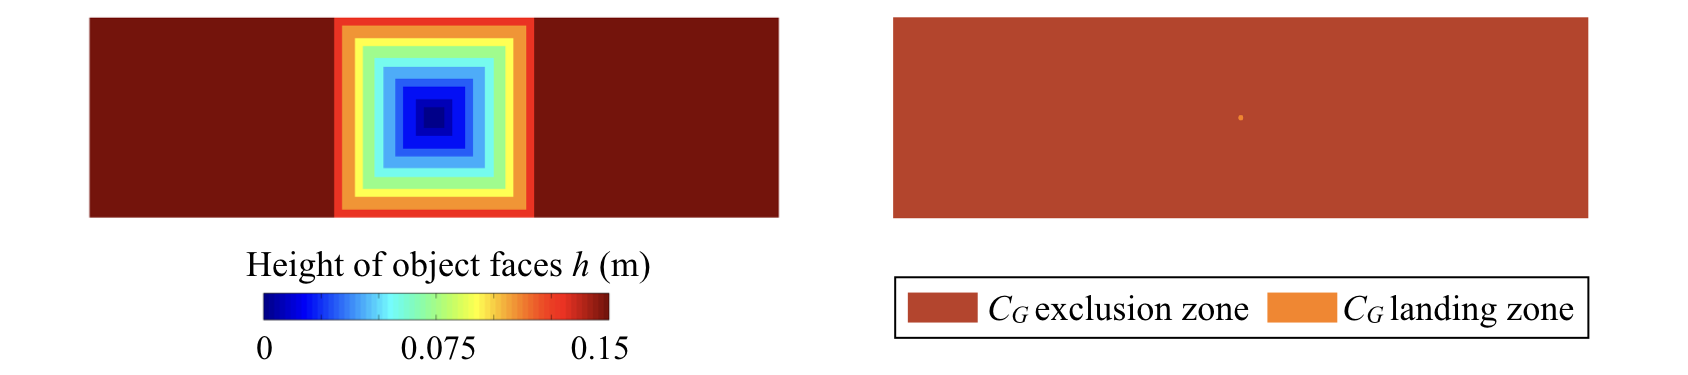
\includegraphics[width=6in]{./images/mehul22a.png}
\caption{Area equal to the landing footprint of the vehicle with possible height values with the centre as landing zone}
\label{f:mehul22a}
\end{figure}
 
 Landing cost $C_s$ is calculated for each site as the average of the three extracted site properties:
 
 \begin{equation}
 \label{eq:eq13}
	C_s = \frac{1}{3}\left[P_s + P_f + P_r \right]
\end{equation} 

Landing costs calculated for the three sites for landing heading $55^\circ$ are seen in Table~\ref{t:table4}. The final landing site for this heading is selected as the one with least landing cost, in this case site C.
   			
\begin{table}[!ht]
\centering
\caption{Landing site properties}
\begin{tabular}{  |p{2cm} p{2cm} p{2cm} p{2cm} p{2cm}| }
\hline
\textbf{Site} & \textbf{$P_s$} & \textbf{$P_f$} & \textbf{$P_r$} & \textbf{$C_s$}\\ \hline 
$A$ & $0.54$ & $0.85$ & $0.29$ & $0.56$ \\
$B$ & $0.67$ & $0.62$ & $0.32$ & $0.54$ \\
$C$ & $0.34$ & $0.65$ & $0.15$ & $0.38$ \\
\hline
\end{tabular}
\label{t:table4}
\end{table}

\subsection{Selecting final landing site}

To select a final landing site for the mapped bathymetry, we need to analyze landing sites along different landing headings. The landing site with the least landing cost can be along any landing heading depending on the vehicle geometry and the seafloor terrain. Landing sites are identified for landing headings between $-90^\circ$ and $90^\circ$ in steps of $5^\circ$. Landing sites along the opposite headings are identical due to the rectangular nature of the structural element. The landing costs calculated for all the landing candidates are seen in Fig.~\ref{f:mehul23}. The landing site $B$ for landing heading $40^\circ$ has the least landing cost and selected as the final landing candidate. The properties for final landing candidate are as in Table ~\ref{t:table5}.


\begin{figure}[!ht]
\centering
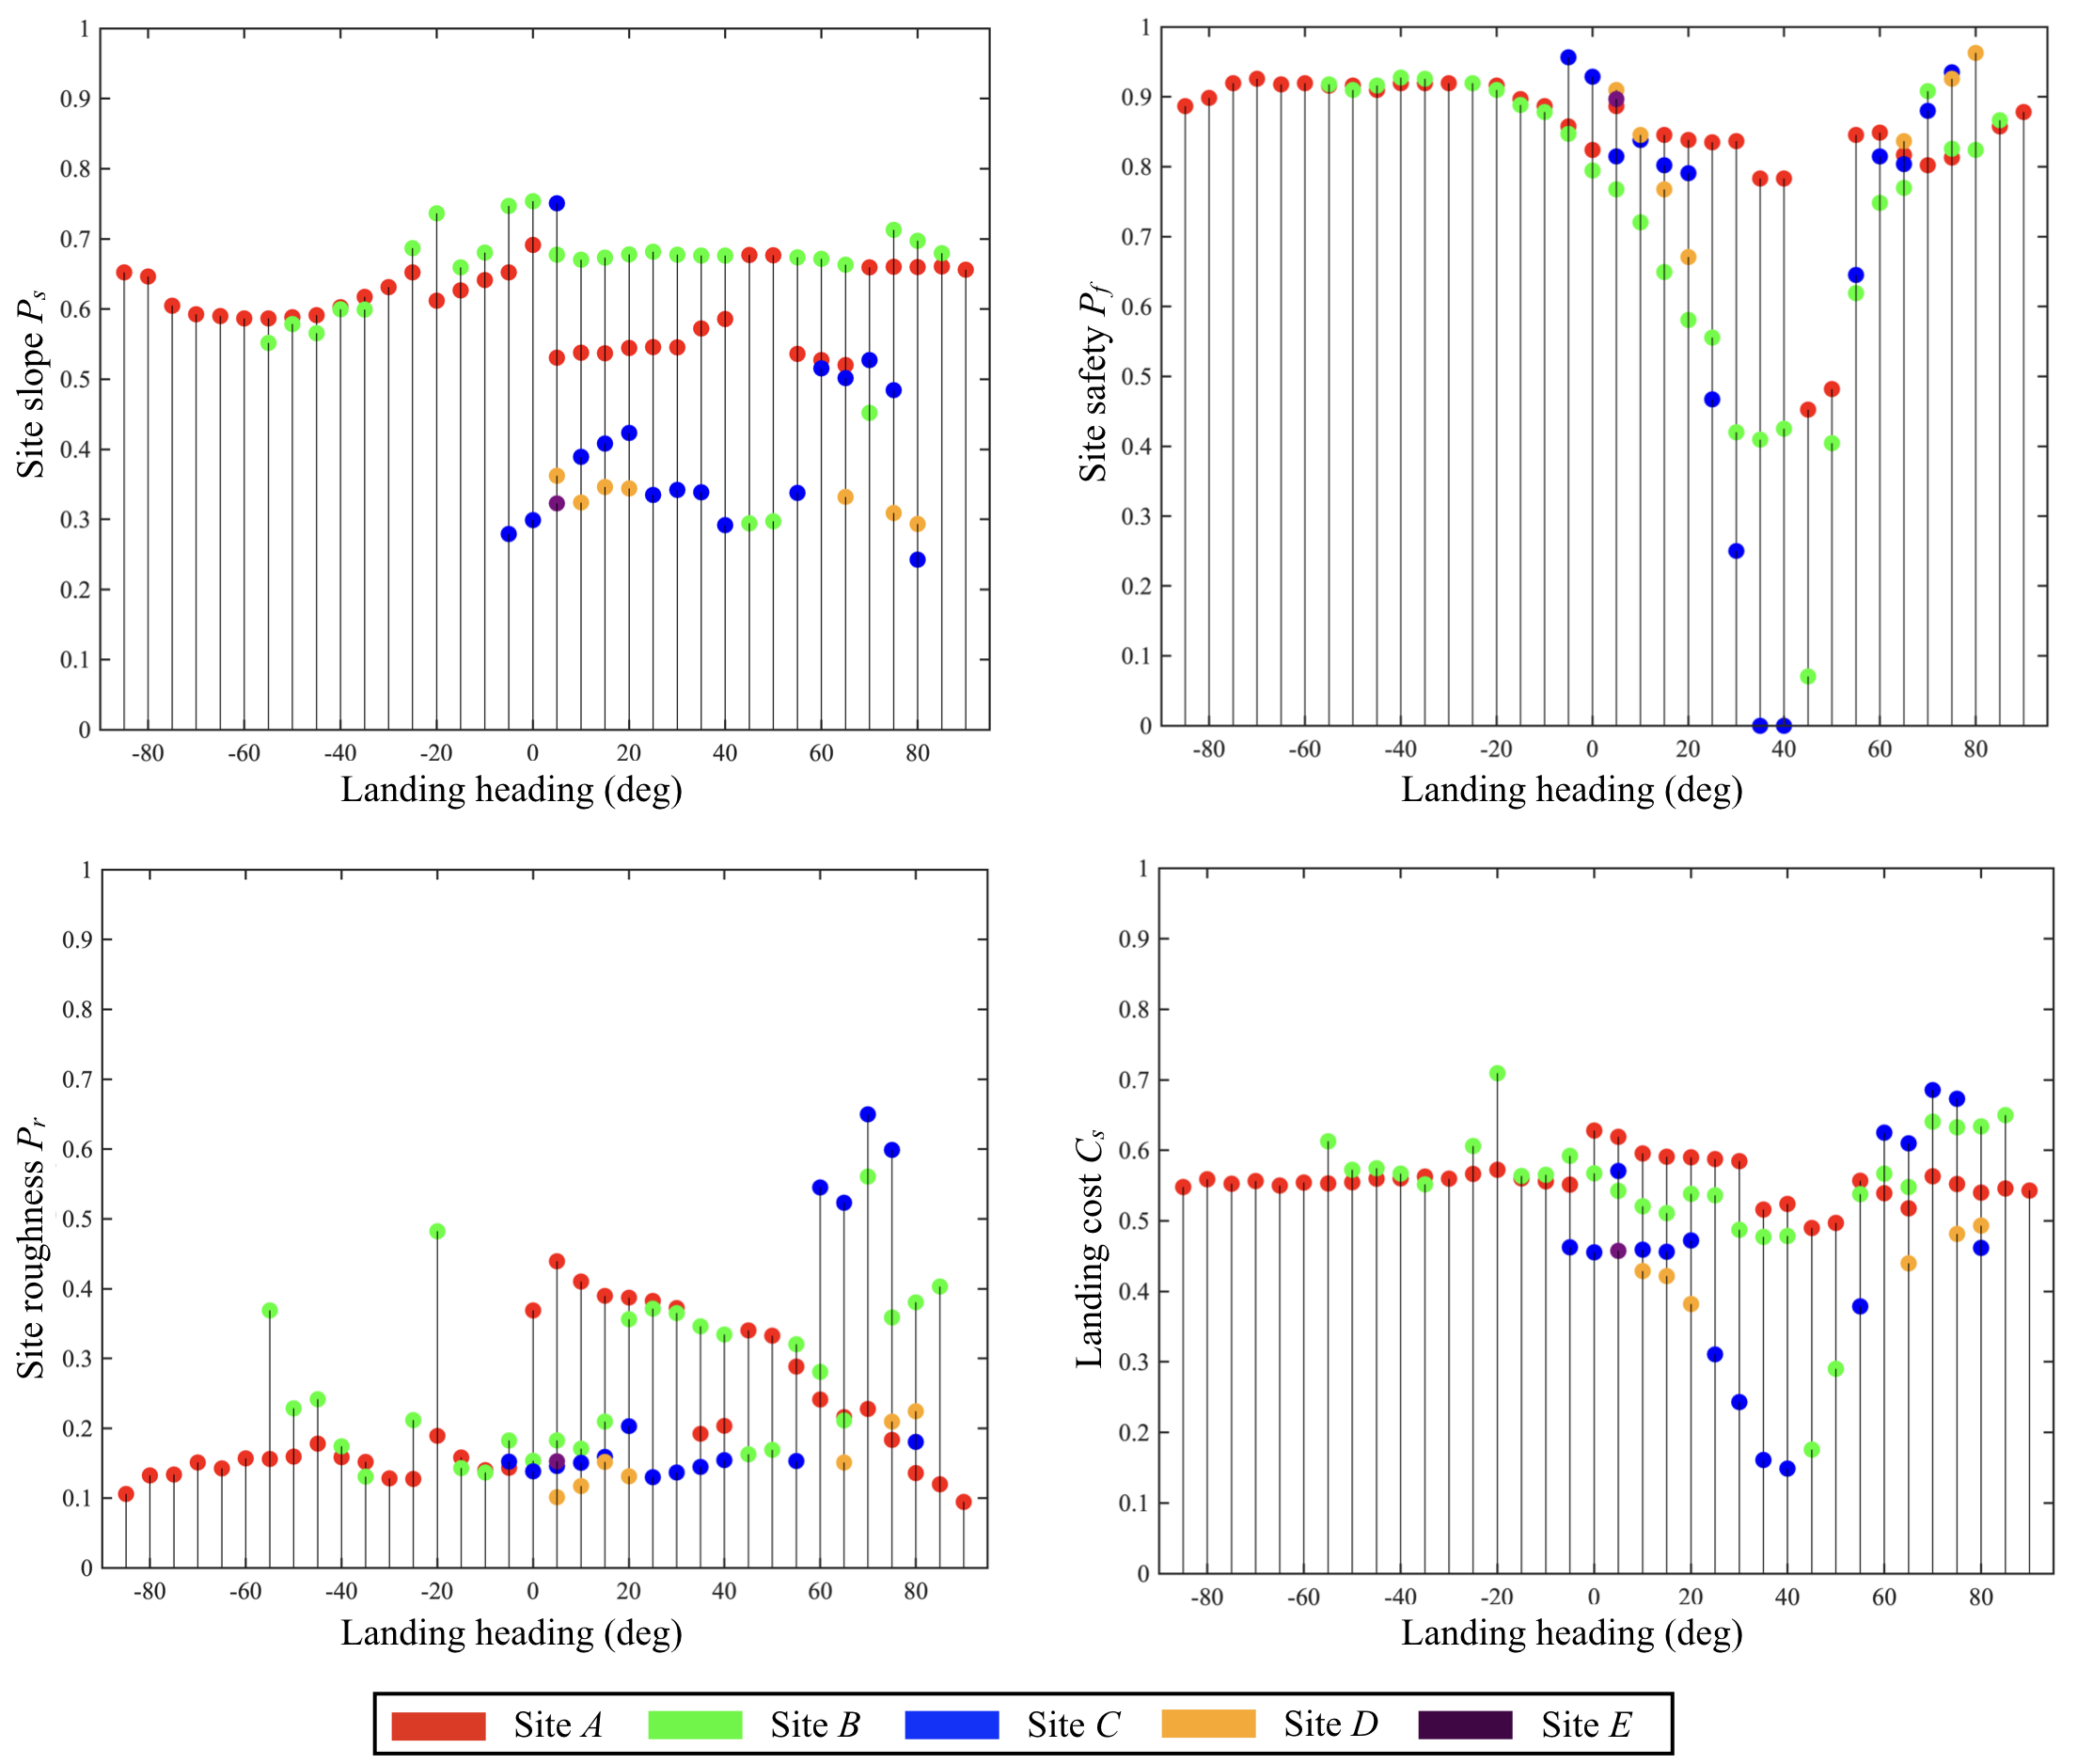
\includegraphics[width=\textwidth]{./images/mehul23.png}
\caption{Properties of the landing sites}
\label{f:mehul23}
\end{figure}


\begin{table}[!ht]
\centering
\caption{Properties for final landing site}
\begin{tabular}{  |p{6cm}  p{4cm}| }
\hline
\textbf{Property} & \textbf{Value}\\ \hline 
Landing heading & $40^\circ$ or $220^\circ$ \\
Mean depth & $1379.72$ m\\
$P_s$ & $0.29$\\
$P_f$ & $0.00$\\
$P_r$ & $0.16$\\
$C_s$ & $0.15$\\
\hline
\end{tabular}
\label{t:table5}
\end{table}


%************************Simulation*******************************

\section{Implementation on seafloor data}

The landing algorithm is applied to a $500$\,m section of high resolution seafloor laser bathymetry data collected on the southern slopes of the Takuyo Daigo seamount between depth of 1379 and 1429\,m. The data was obtained by the AUV BOSS-A using the same mapping system described in Section ~\ref{sec:algo}. In order to perform the analysis, the data is split into twenty $25$\,m long submaps as illustrated in Fig~\ref{f:mehul24}. The northern part of the transect (submaps 1 to 9) is gently sloped with relatively flat, exposed manganese crusts. The  southern parts of the transect (submaps 10 to 20) is more steeply sloped with a higher degree of rugosity~\cite{Thornton2013l,Bodenmann2016}. The algorithm was applied to determine the most appropriate landing coordinate and heading within each submap for the vehicle parameters given in Table~\ref{t:table2}. 

	
\begin{figure}[!ht]
\centering
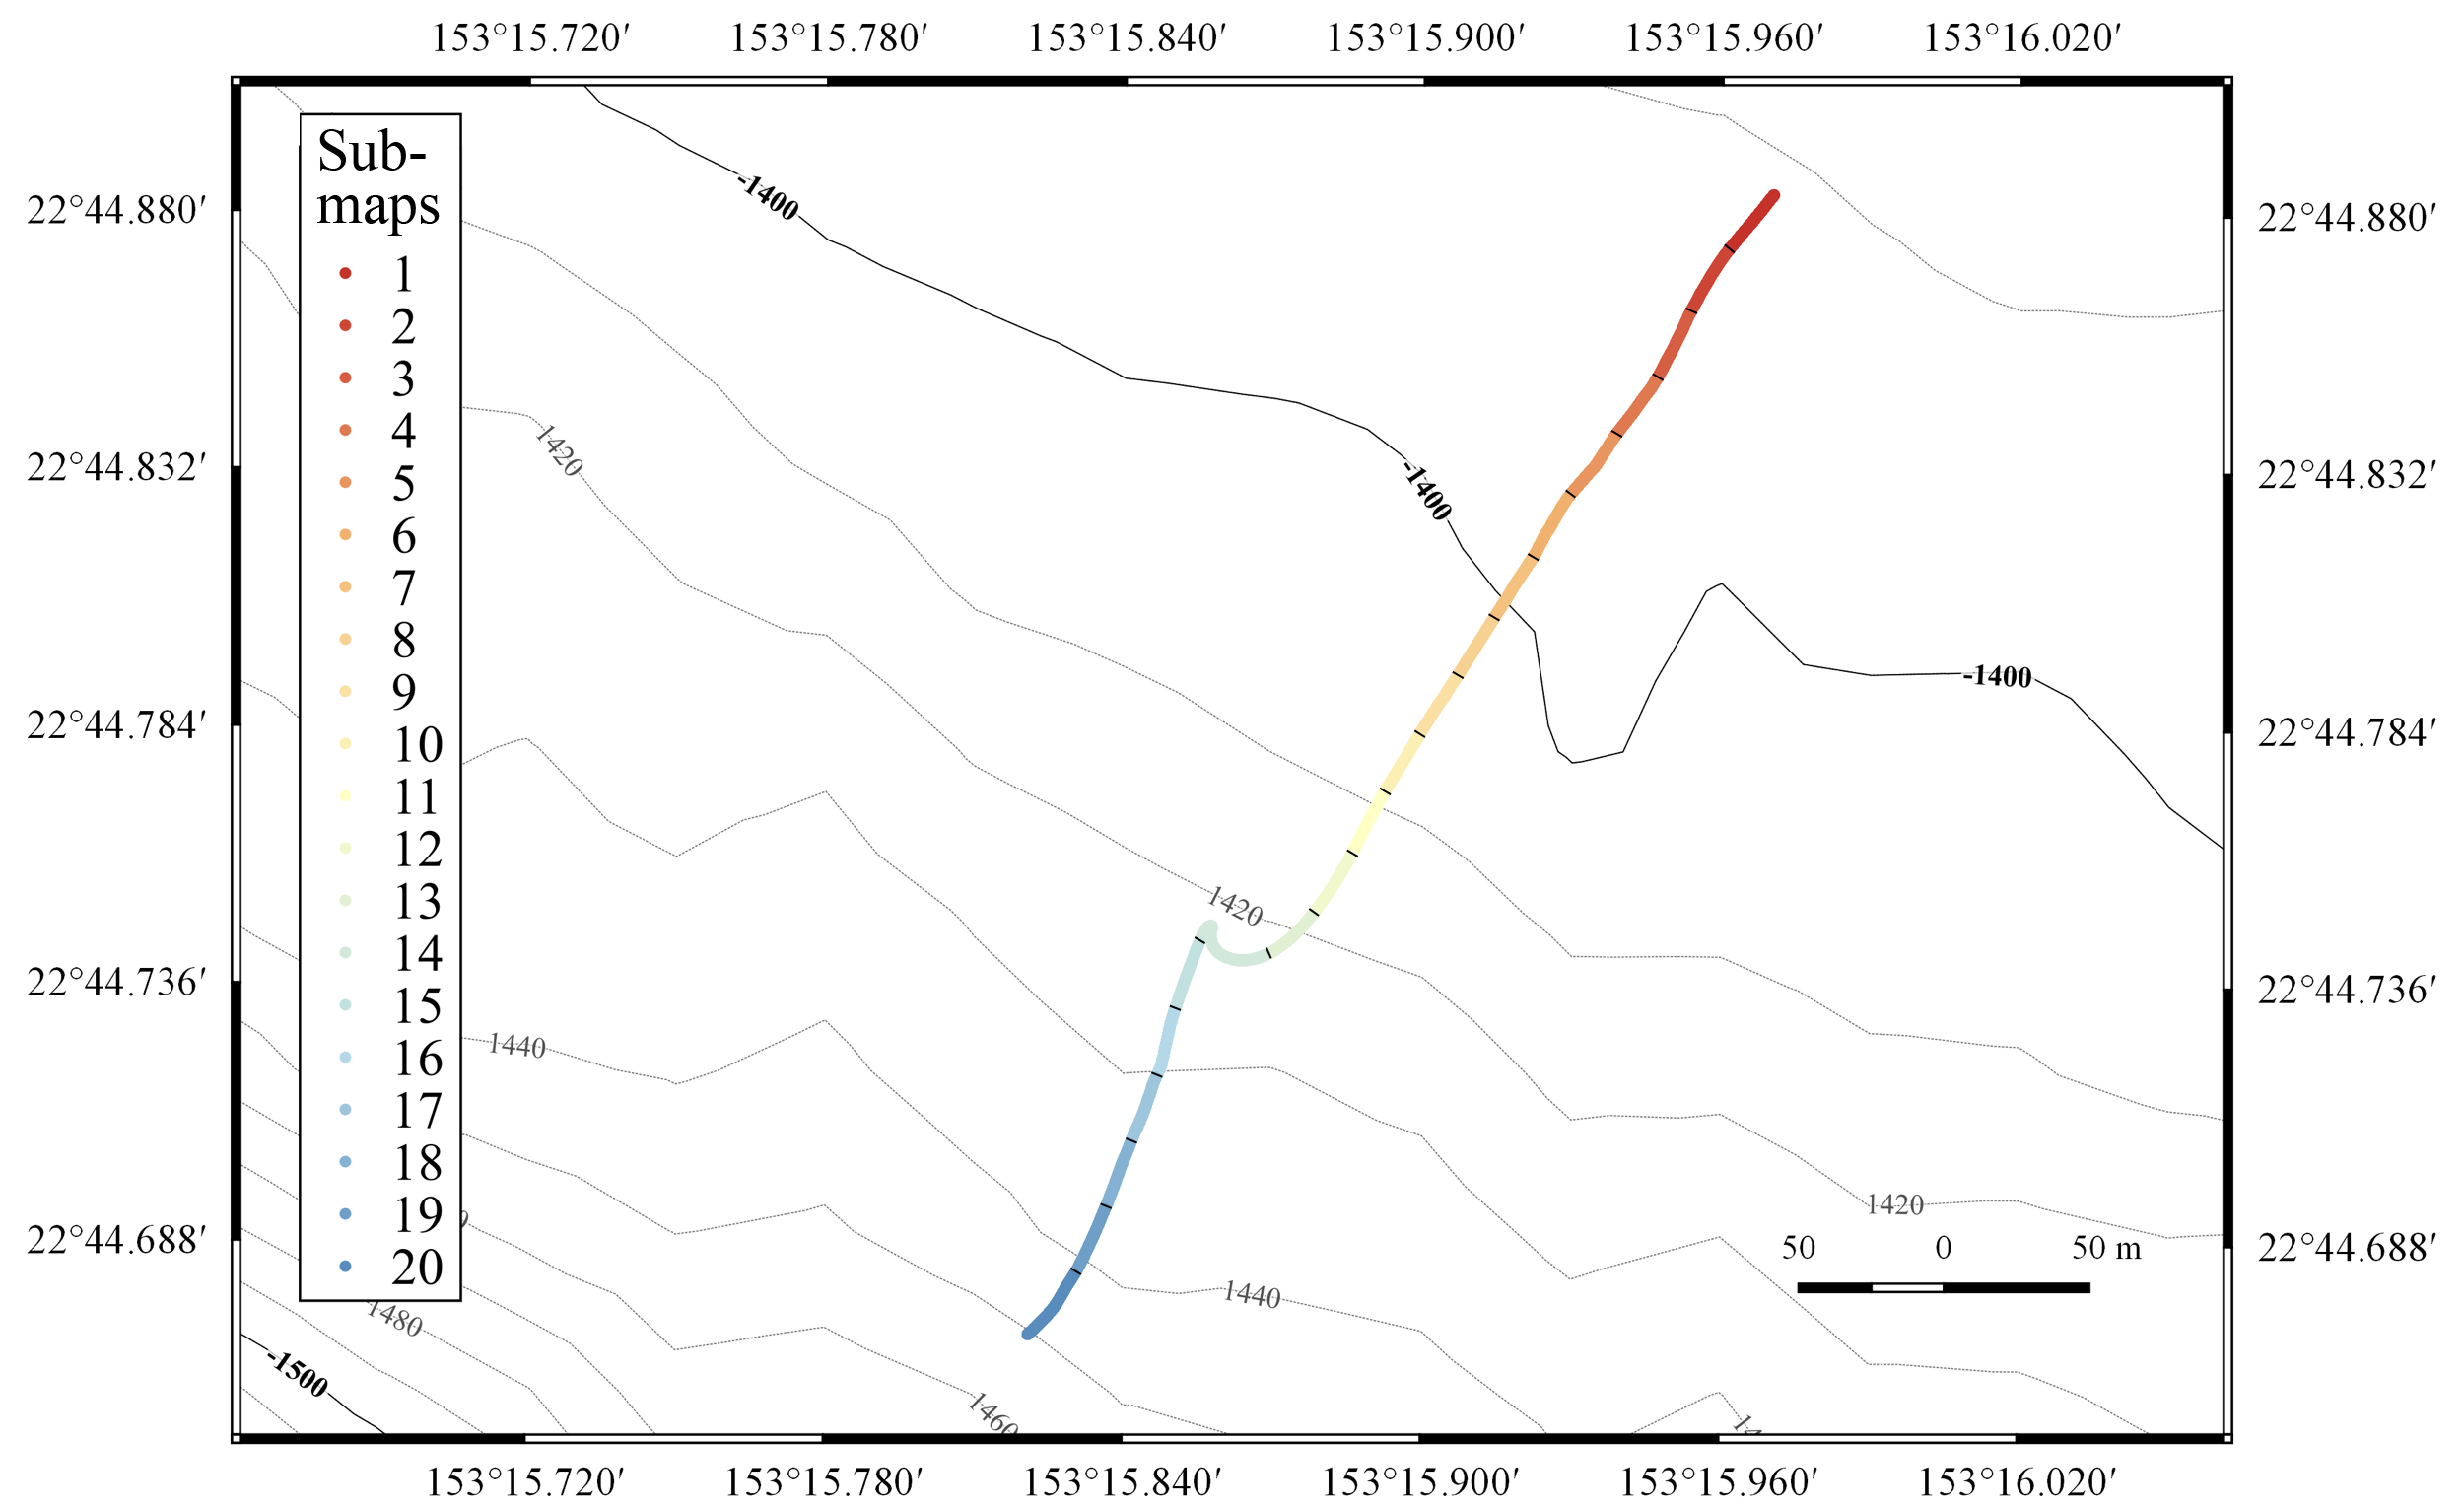
\includegraphics[width=6.5in]{./images/mehul24_BT.png}
\caption{Vehicle trajectory at Takuyo Daigo seamount where the algorithm is implemented on twenty $25$\,m long submaps}
\label{f:mehul24}
\end{figure}

\begin{figure}[!ht]
\centering
\subfloat[Properties and landing costs determined for the sites selected within each submap\label{sf:mehul25}]{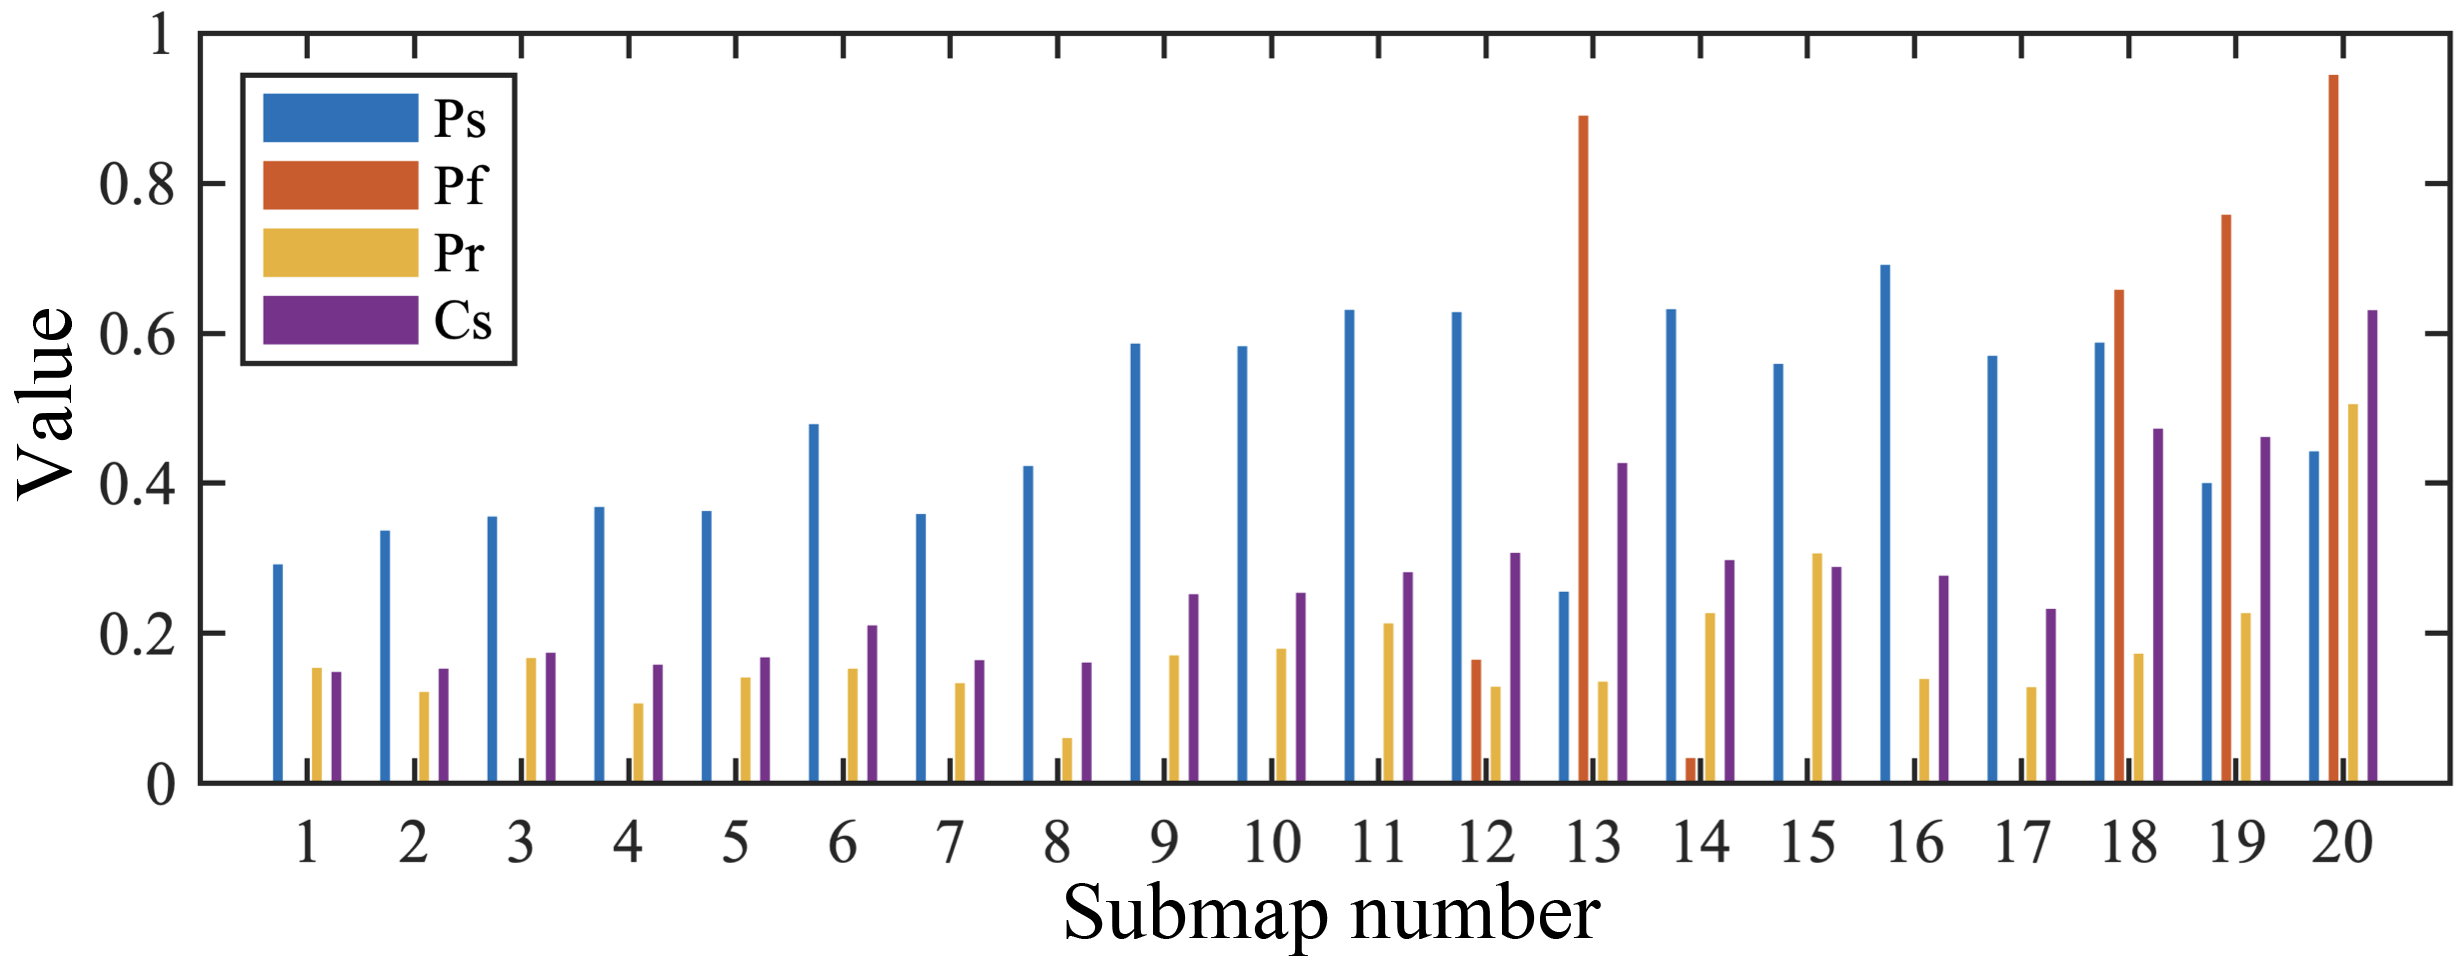
\includegraphics[width=5.5in]{./images/mehul25_BT.png}}\quad
\subfloat[Landing headings for the sites selected within each submap\label{sf:mehul26}]{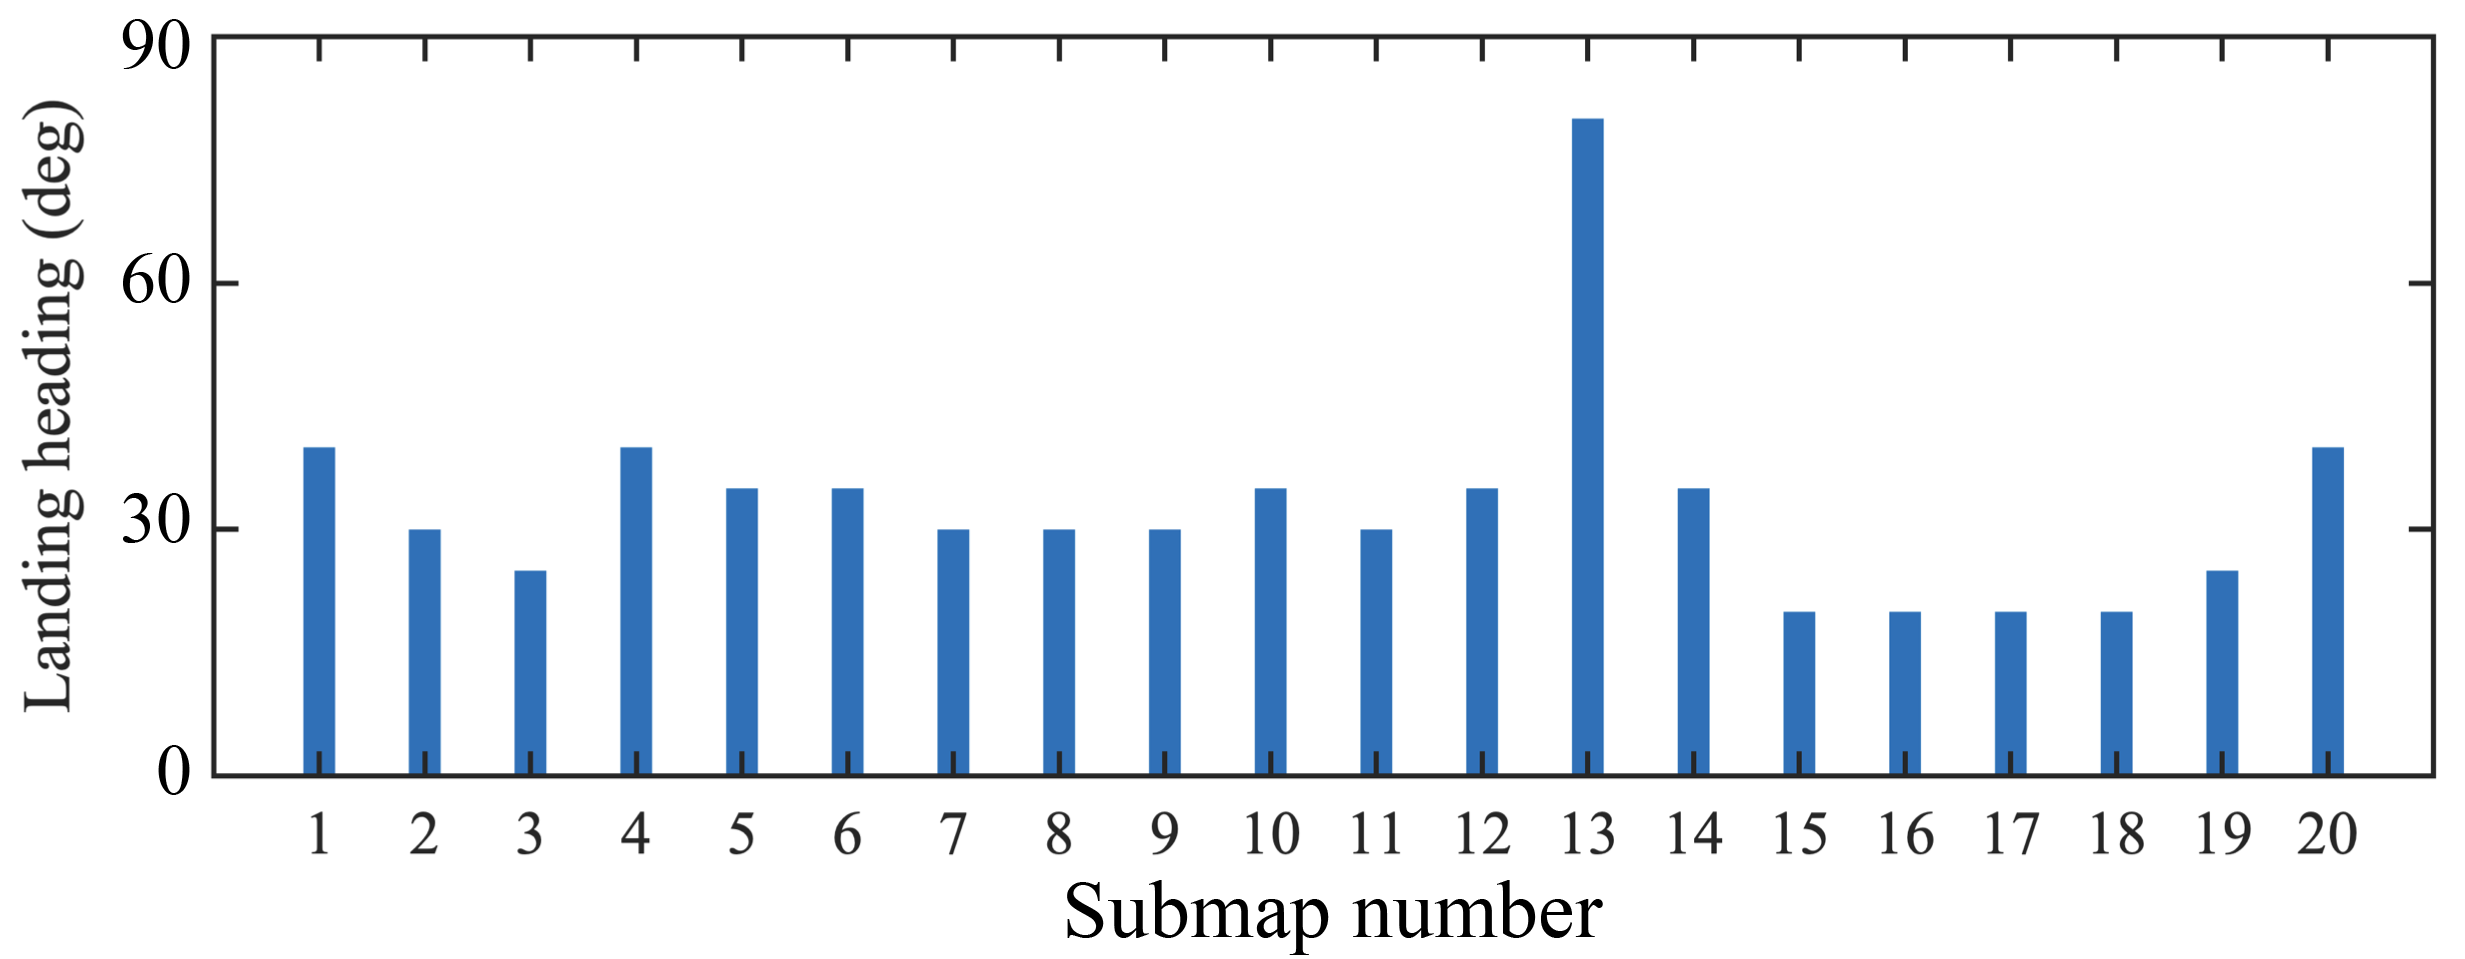
\includegraphics[width=5.5in]{./images/mehul26_BT.png}}
\caption{Characteristics of the landing sites determined by the algorithm for the submaps analysed in this work.}
\end{figure}

The algorithm selected landing sites in each submap, the properties of which can be seen in Fig~\ref{sf:mehul25}. The landing heading for each patch is close to the mapping heading due to the narrow swath of the bathymetry as shown by Fig~\ref{sf:mehul26}. This is clearly visible for the submaps shown in Fig~\ref{f:mehul27}. The sites towards the south of the transect (submaps 10 to 20) have higher landing costs than the transects towards the north of the transect (submaps 1 to 9) with larger values of Ps and Pr due to the increased steepness and rugosity. Fig~\ref{f:mehul27}a shows Submap $XX$, which has a low landing cost due to the wide swath and gently sloping smooth surface. Submap $YY$ (Fig~\ref{f:mehul27}b) shows a narrow landing area due to reduced mapping swath while turning on an smooth, gently sloping area of the seafloor. Submap $ZZ$ (Fig~\ref{f:mehul27}c) towards the lower end of the transect has a narrow landing area on an area with high rugosity and a steep slope, resulting in a high landing cost. Fig~\ref{f:mehul28} shows the locations of each landing site identified in the submaps with their Cs values.

\begin{figure}[!ht]
\centering
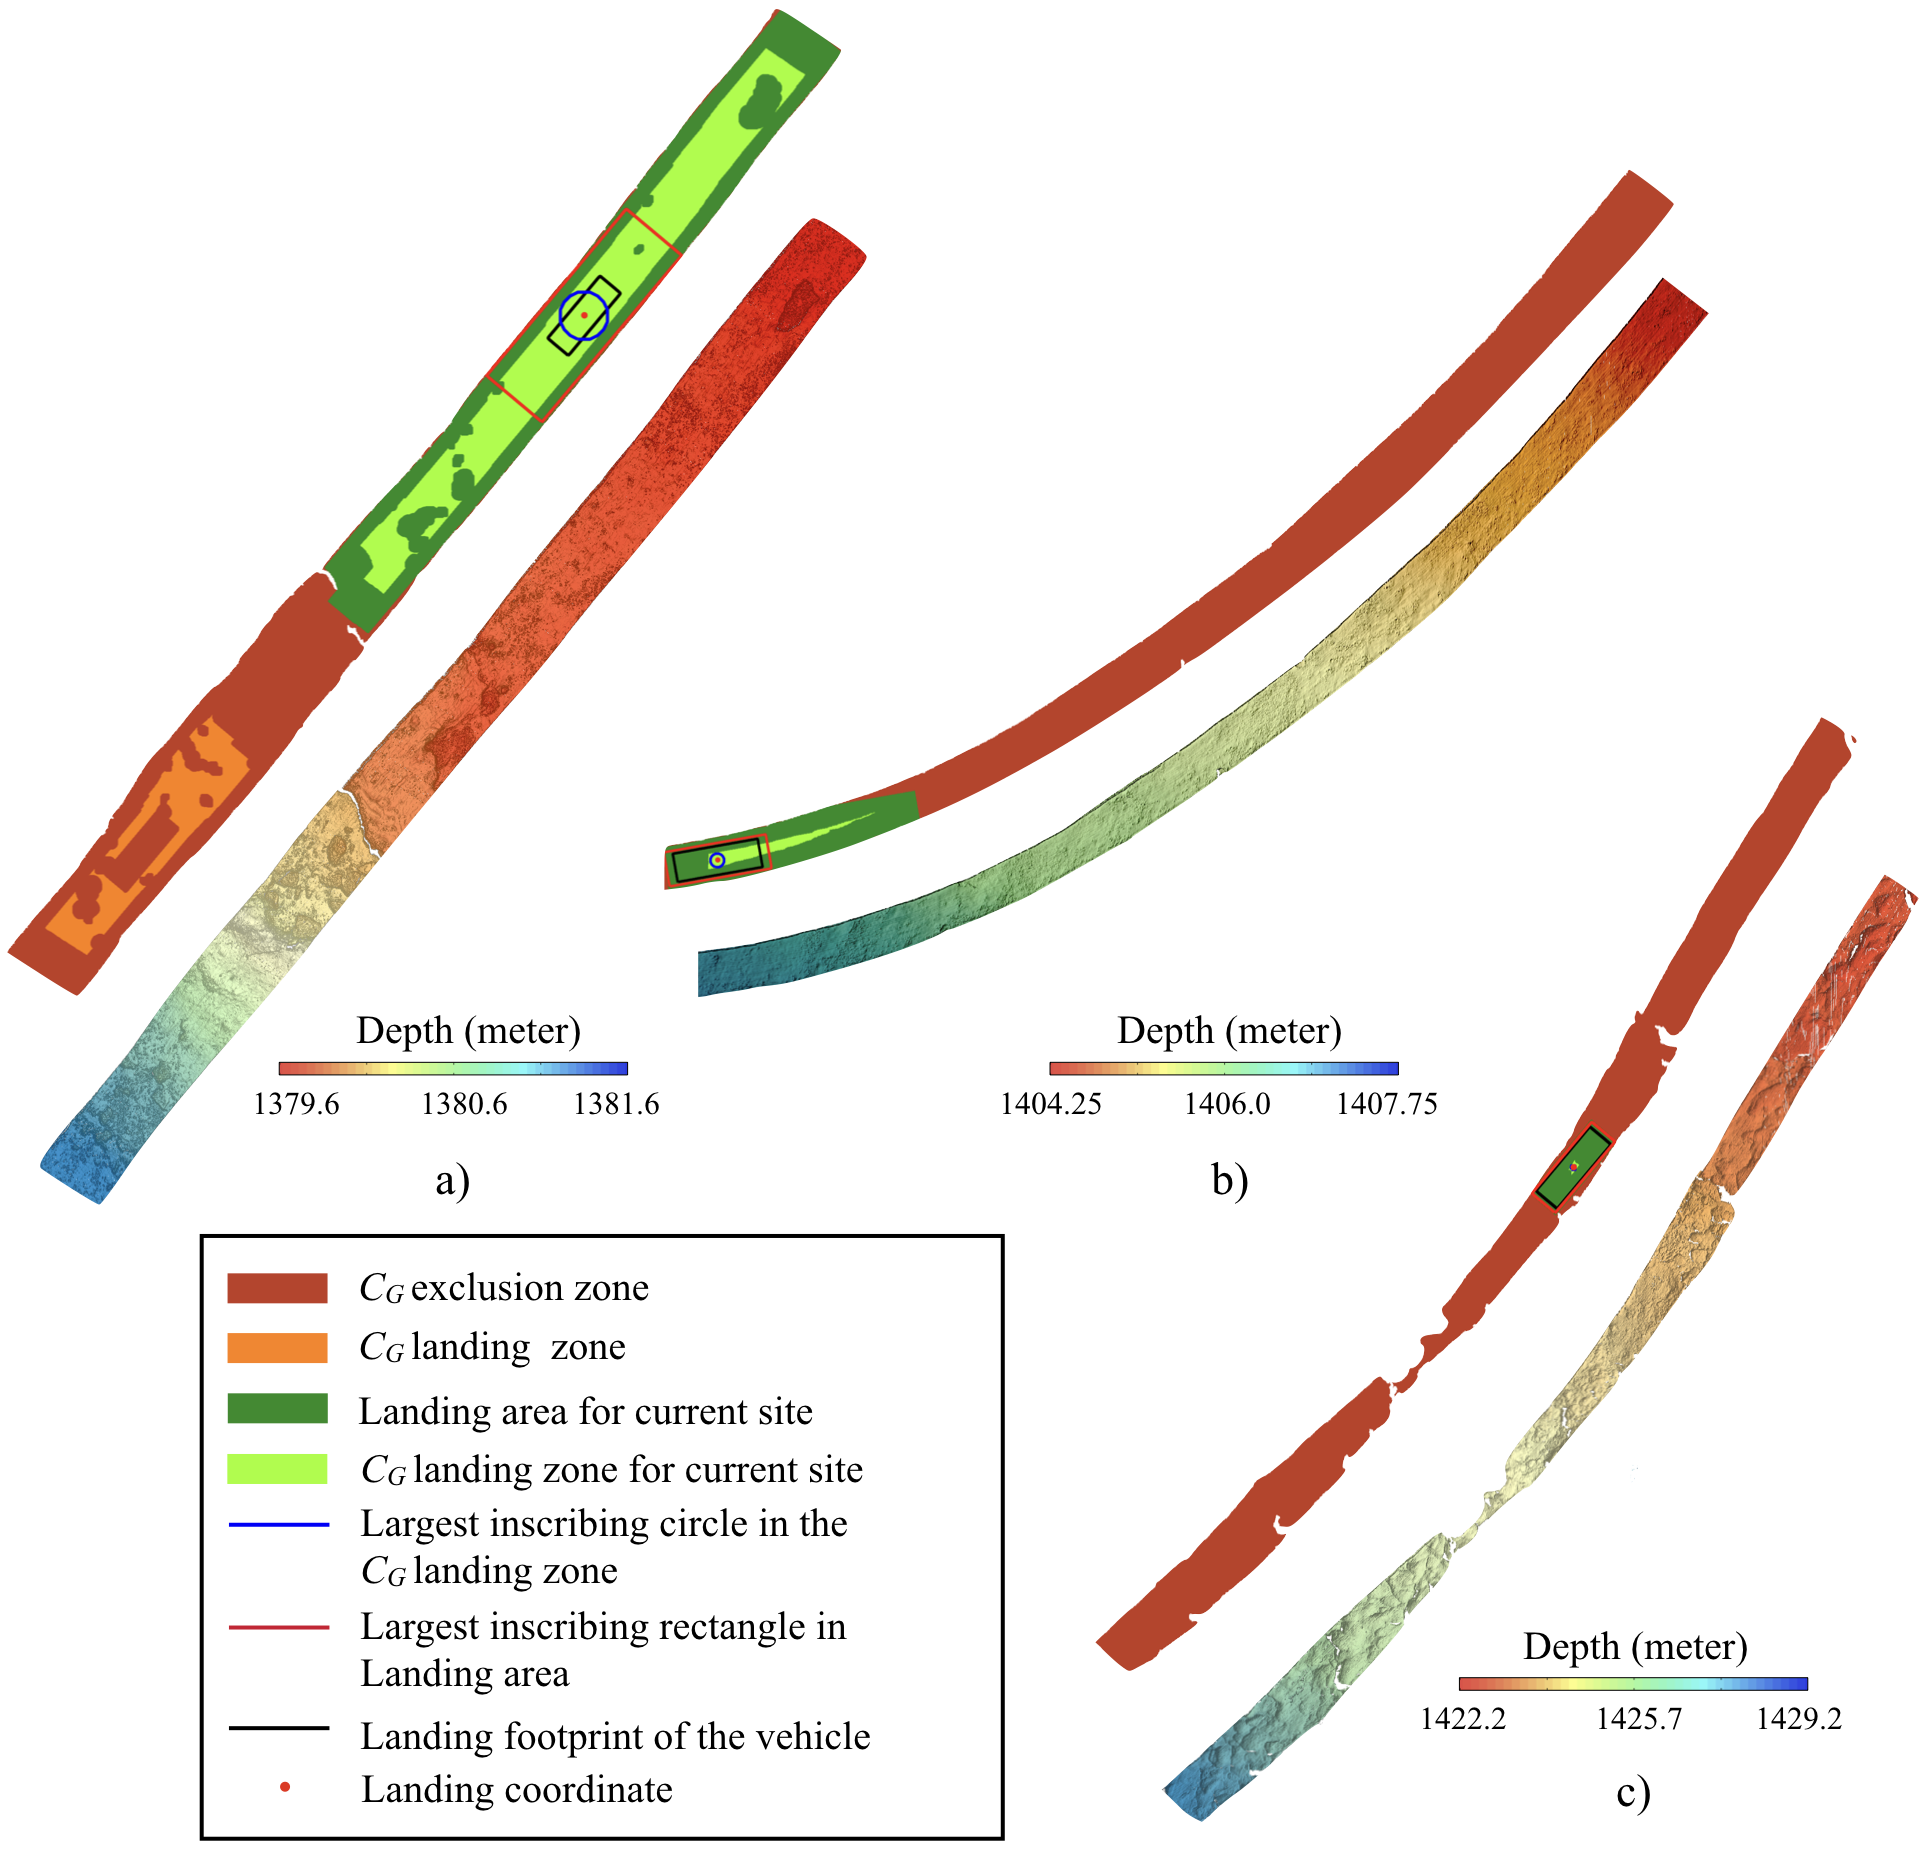
\includegraphics[width=\textwidth]{./images/mehul28.png}
\caption{Landing cost for sites identified}
\label{f:mehul27}
\end{figure}

\begin{figure}[!ht]
\centering
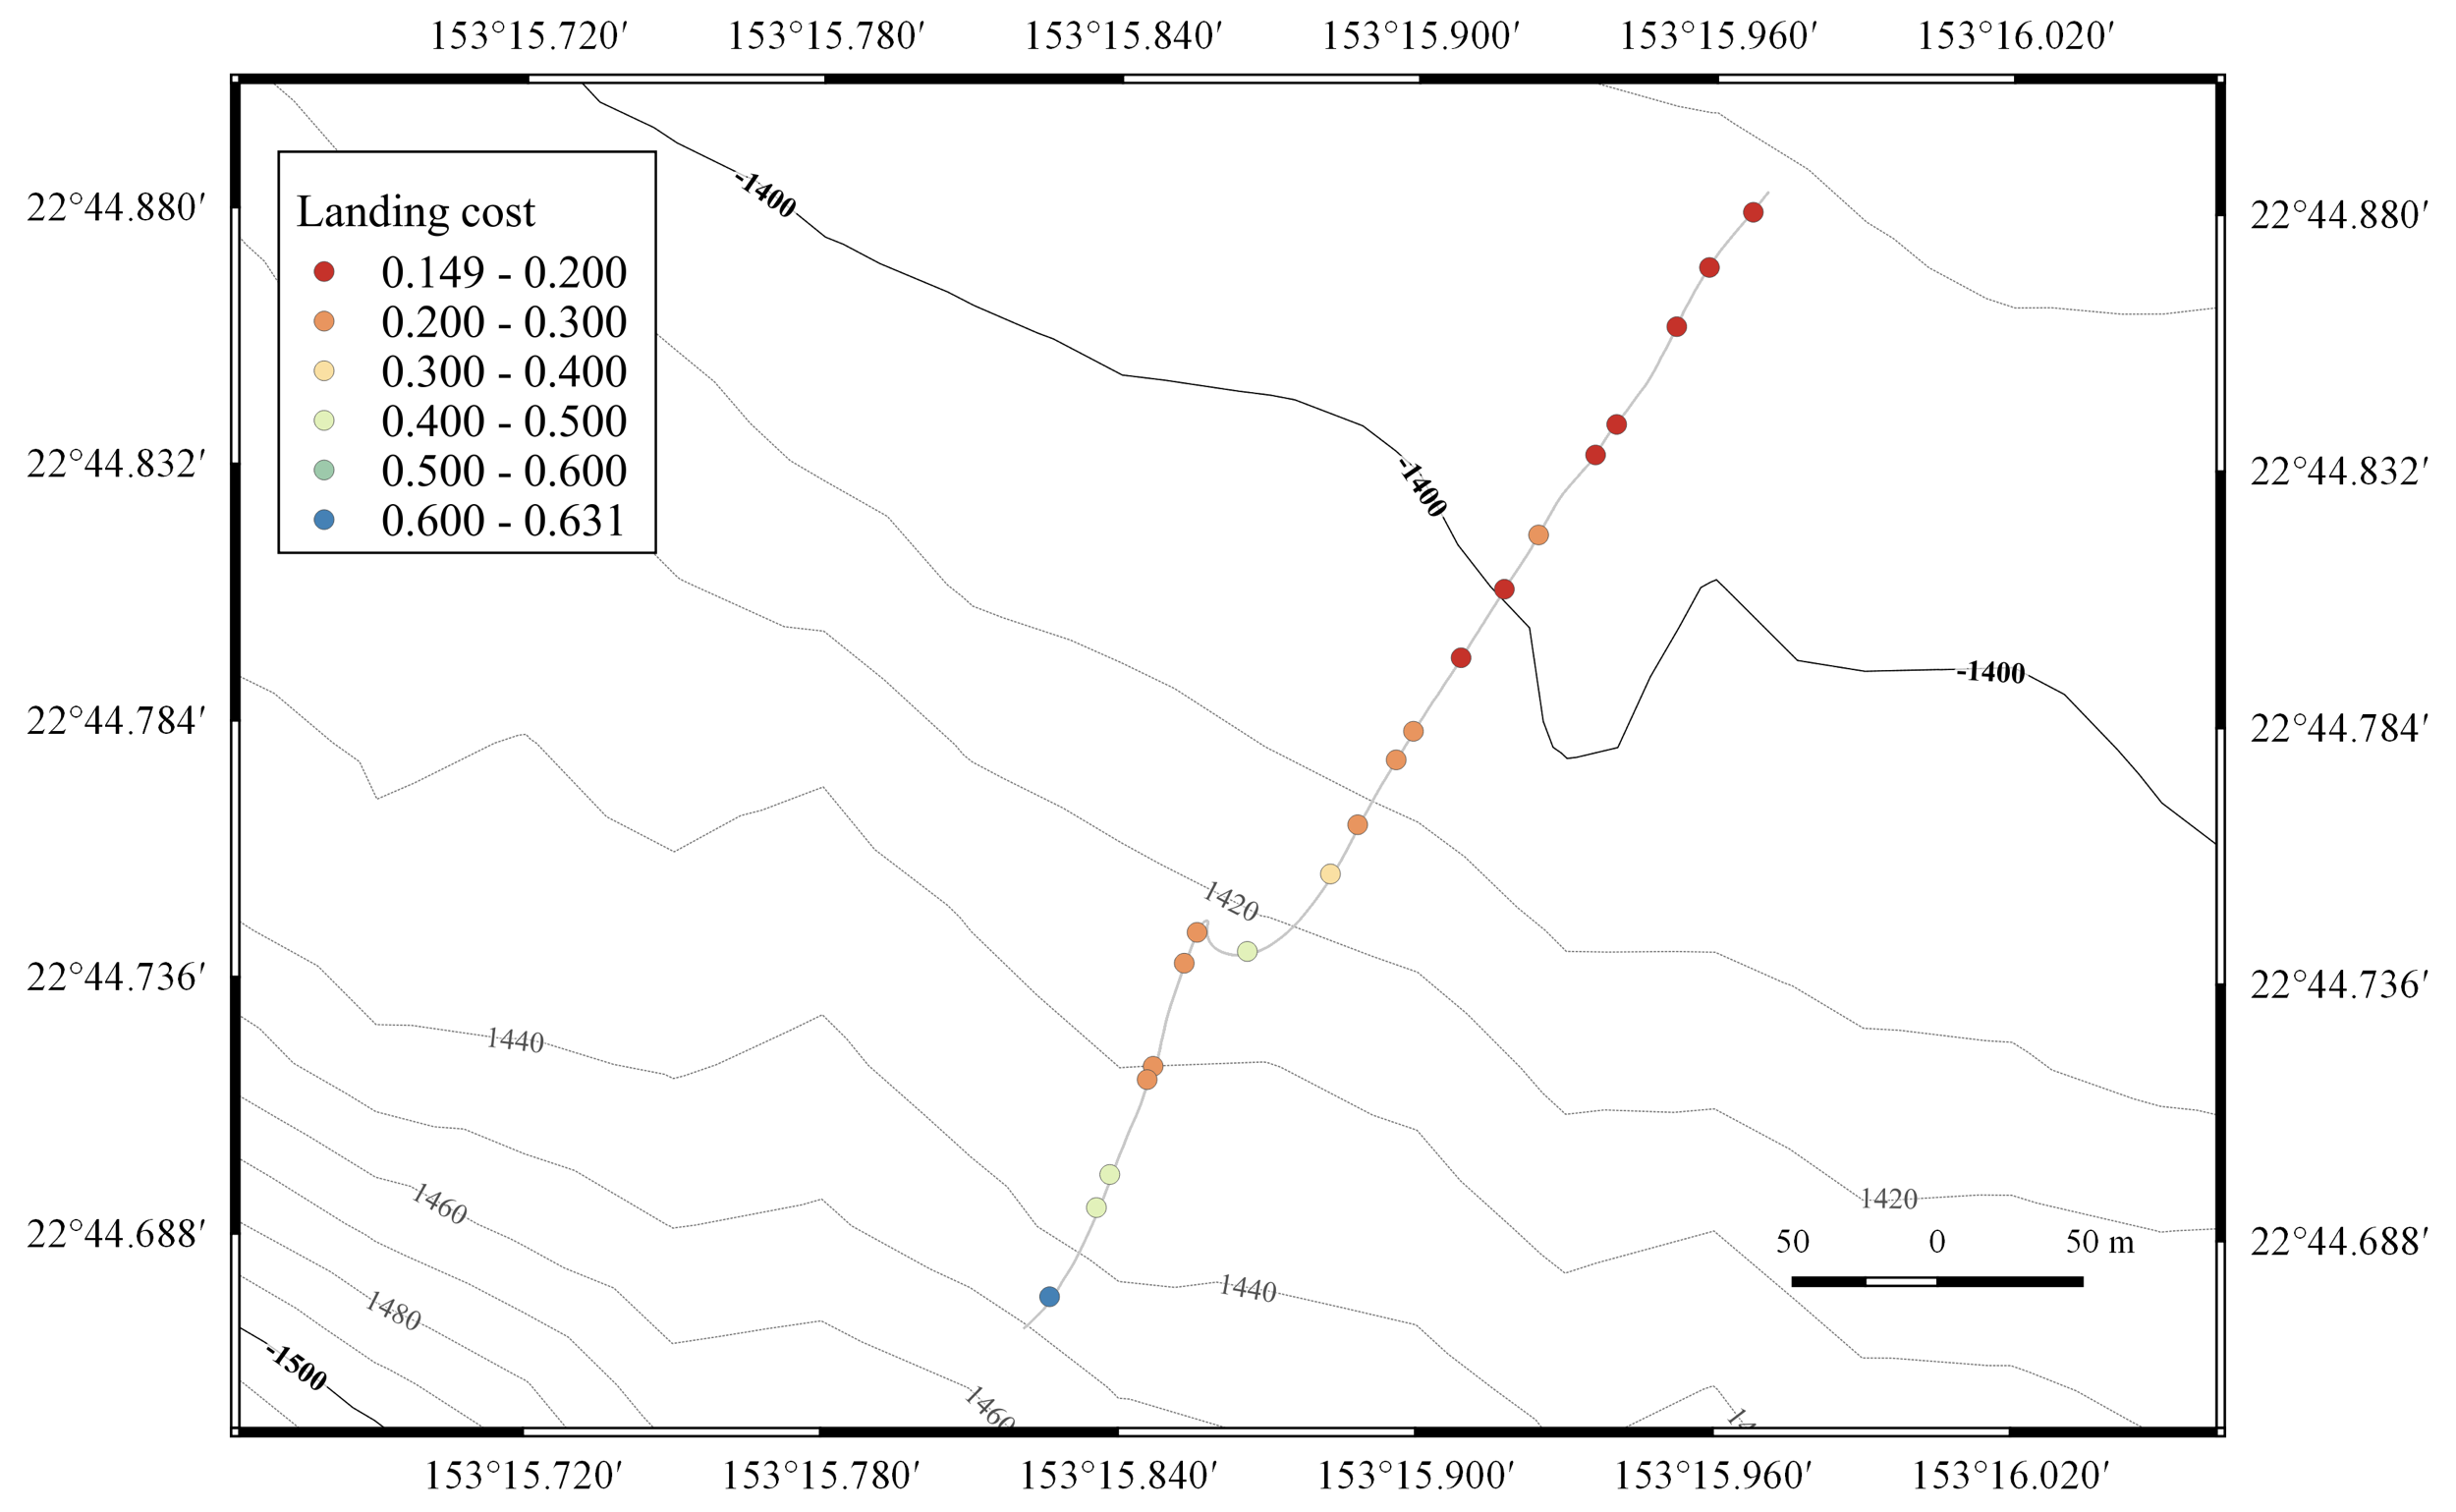
\includegraphics[width=6in]{./images/mehul27.png}
\caption{Landing cost for sites identified}
\label{f:mehul28}
\end{figure}

\begin{table}[!ht]
\centering
\caption{Results of analysis on mapped bathymetry}
\begin{tabular}{  |c c c c c|}
\hline
\textbf{Area surveyed} & \textbf{Number of sites} & \textbf{Mean landing cost} & \textbf{Landing cost range} & \textbf{Landing cost Std. Dev.}\\ \hline 
$794.4$ sq.m. & $754$ & $0.28$ & $0.15 - 0.63$ & $0.13$ \\
\hline
\end{tabular}
\label{t:table6}
\end{table}

%%**********************Conclusions******************

%%*************************************************************************
\section{Conclusions}

This study presents a novel, fully automated method to identify safe landing sites on the based on mm-resolution seafloor bathymetry. The conditions that need to be satisfied for safe landing considering the seafloor terrain and vehicle geometry have been derived and these are used to allow an autonomous platform to identify and select landing sites based on a cost function. The method is applied to seafloor data acquired using high resolution laser bathymetry along a transect of $500$\,m, successfully identifying and selecting landing coordinates and headings. The computational times demonstrate that the calculations are applicable to in mission operations from an AUV and that the approach can enable autonomous platforms to use in-situ sensors that require a vehicle to have landed for their operations. Vehicle hardware and seafloor mapping system considerations specific to autonomous landing are described and the concept of a negatively buoyant, fast transiting landing vehicle are presented.

%%*************************************************************************

\section*{Acknowledgments}

The authors would like to thank Y. Nishida of Kyushu Institute of Technology, K. Nagahashi and K. Nagano of Mitsui Engineering and Shipbuilding, U. Neettiyath of The University of Tokyo and T. Koike of Kaiyo Engineering for their help in deployment of BOSS-A during the KR$16-01$ cruise of R/V Kairei. This work was funded under the Program for the Development of Fundamental Tools for the Utilization of Marine Resources of the Japanese Ministry of Education.


%%*************************************************************************

\bibliographystyle{IEEEtran}
\bibliography{articles}

%%************************IEEEbiography*********************************

\begin{IEEEbiography}[{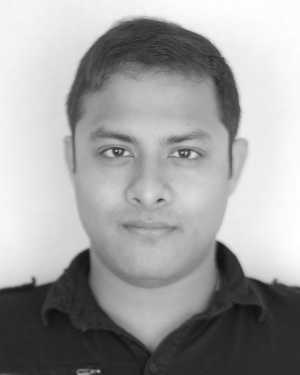
\includegraphics[width=1in,height=1.5in,clip,keepaspectratio]{./images/sange.png}}]{Sangekar Mehul Naresh}
(M’10) received the M.Sc. degree in underwater robotics and Ph.D. degree in ocean technology from The University of Tokyo, Japan, in 2010 and 2014, respectively. He is  working at present as a project researcher at the Thornton Lab, Institute of Industrial Science, The University of Tokyo. Currently, he works on techniques for intelligent, multi-layer resolution mapping of the seafloor using autonomous underwater vehicles. He is also working on developing algorithms for analysis of high resolution seafloor bathymetry and correlating it with other measured seafloor parameters.  
\end{IEEEbiography}

\vskip 0pt plus -1fil

\begin{IEEEbiography}[{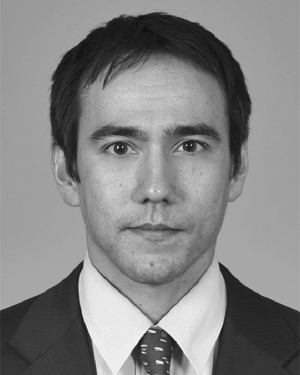
\includegraphics[width=1in,height=1.5in,clip,keepaspectratio]{./images/thorn.png}}]{Thornton Blair}
(M’07) received the B.Eng. degree in ship science and the Ph.D. degree in underwater robotics from The University of Southampton, Southampton, U.K., in 2002 and 2006, respectively. He is at present an Associate Professor at the the University of Southampton and also affiliated with the  Ocean Perception Laboratory, Institute of Industrial Science, The University of Tokyo. His research interests involve the development of in-situ sensors and data processing techniques for integrated acoustic, visual, and chemical survey of marine minerals and environment monitoring. He is dedicated to fielding real systems in real environments and overcoming bottlenecks in the flow of information from data collection to human interpretation.
\end{IEEEbiography}

\vskip 0pt plus -1fil

\begin{IEEEbiography}[{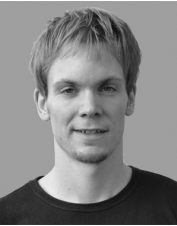
\includegraphics[width=1in,height=1.5in,clip,keepaspectratio]{./images/boden.png}}]{Adrian Bodenmann}
(M’09) received the M.Sc. degree in microengineering from the Ecole Poly- technique Fédérale de Lausanne (EPFL), Lausanne, Switzerland, in 2009. He is a Project Researcher at the Underwater Technology Research Center, University of Tokyo, Tokyo, Japan. Currently, he works on 3-D seafloor visual mapping and automated data processing algorithms, and is developing a long-range 3-D color mapping system for wide area marine surveys.
\end{IEEEbiography}

\vskip 0pt plus -1fil

\begin{IEEEbiography}[{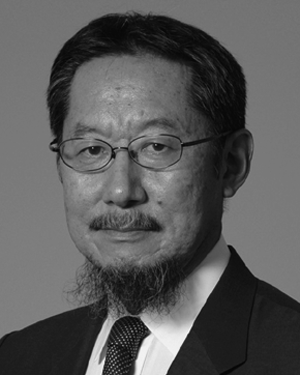
\includegraphics[width=1in,height=1.5in,clip,keepaspectratio]{./images/ura.png}}]{Ura Tamaki}
(M’91–SM’02–F’07) graduated from the Faculty of Engineering, The University of Tokyo, Japan, in 1972 and received the degree of Doctor of Engineering from the same university in 1977. He is at present the Professor emeritus of The University of Tokyo and  Director, Distinguished Professor of Center for Socio-Robotic Synthesis, Kyushu Institute of Technology, and Director of Underwater Technology Center of National Maritime Research Institute. He has developed various types of Autonomous Underwater Vehicles (AUVs) and related application technologies including navigation methods, a new sensing method using a chemical sensor, precise seafloor mapping methods, a precise seabed positioning system with a resolution of a few centimeters, a new sensing system of the thickness of cobalt-rich crust, etc. Finally, he exemplified using these technologies that AUVs are practicable and valuable tools for deep-sea exploration.
\end{IEEEbiography}

\end{document}

%%*************************************************************************